\documentclass[preprint,12pt]{elsarticle}

\journal{Neural Networks}

\usepackage{amsmath,amssymb}
\usepackage{graphicx}

\usepackage{array}
\usepackage{multirow}
\usepackage[T1]{fontenc}
\usepackage{xurl}
\usepackage[hidelinks,unicode]{hyperref}
\usepackage{tabularx}
\usepackage{booktabs}

\usepackage{float}
\usepackage[section]{placeins}
\usepackage{lineno}
\usepackage{algorithm}
\usepackage{algpseudocode}
\usepackage{microtype}

\setlength{\emergencystretch}{3em}
\Urlmuskip=0mu plus 2mu\relax

\newcolumntype{Y}{>{\raggedright\arraybackslash}X}
\newcolumntype{C}{>{\centering\arraybackslash}X}


\hyphenation{
task-incremental
class-incremental
gate-correctness
self-scored
continual-learning
replay-based
ResNet
CIFAR
}

\graphicspath{{figs/}}

\biboptions{numbers,sort&compress}

\begin{document}

\begin{frontmatter}

\title{Reliability-Gated Replay Reveals a Power--Safety Frontier for Unreliable Data in Continual Learning}

\author[inst1]{Marlon Malheiros}
\ead{marlon.malheiros1@gmail.com}

\author[inst1]{Antonio Pereira}
\ead{apereira@ufpa.br}

\address[inst1]{Signal Processing Laboratory, Universidade Federal do Par\'a (UFPA), 66075-110 Bel\'em, PA, Brazil}

\begin{abstract}
Experience replay mitigates catastrophic forgetting, but stored samples exert repeated gradient influence and can reinforce unreliable supervision. We study reliability-gated replay as a diagnostic assay for continual learning under label noise. The central question is when replay admission selects useful experience, when it selects corrupted experience, and when memory purification no longer controls accuracy.

Label corruption provides a controlled assay because it exposes sample correctness, buffer purity, and an oracle clean-selector. Across MNIST, CIFAR-10, CIFAR-10N, and CIFAR-100 continual-learning streams, reliability-gated replay exhibits a power--safety frontier. When gate scores remain aligned with true correctness, gated replay purifies the buffer and improves learning. When severe corruption makes the reliability signal anti-aligned, the same admission mechanism stabilizes mislabeled samples, producing gate inversion. Gate--correctness separation predicts replay payoff when memory purity limits performance: Pearson $r=+0.74$ across gated runs, $r=+0.80$ at the condition-mean level, and ROC-AUC $0.85$ for predicting whether gating helps or harms. The predictor becomes uninformative in class-incremental CIFAR, where representational forgetting dominates buffer contamination. Real human-label noise in CIFAR-10N remains in the aligned regime: gates purify the buffer without inverting. An oracle selector isolates the effect of buffer purity and shows that clean selective replay is sufficient to improve learning under the fixed replay mechanism, while the oracle gap quantifies the cost of endogenous self-scoring.

The main result is a diagnostic principle for replay-based continual learning: reliability-gated replay is adaptive when endogenous reliability is aligned with useful experience, maladaptive when it is anti-aligned, and insufficient when representational forgetting rather than memory purity dominates performance.
\end{abstract}

\begin{keyword}
continual learning \sep catastrophic forgetting \sep experience replay \sep label noise \sep sample selection \sep memory purity \sep reliability estimation \sep robustness
\end{keyword}

\end{frontmatter}

\noindent\textbf{Corresponding author:} Antonio Pereira.
Email: \href{mailto:apereira@ufpa.br}{apereira@ufpa.br};
ORCID: \href{https://orcid.org/0000-0002-0808-1058}{0000-0002-0808-1058}.

\vspace{1em}

\linenumbers

\section{Introduction}

Continual learning trains a single model on a sequence of tasks without unrestricted access to earlier data. The central difficulty is catastrophic forgetting: learning a new task can overwrite representations and decision boundaries needed for previous tasks \cite{McCloskey1989Catastrophic,French1999Catastrophic}. Experience replay, which rehearses a small memory of past examples, remains one of the strongest and most architecture-agnostic strategies for mitigating forgetting \cite{LopezPaz2017GEM,Rolnick2019ExperienceReplay,Chaudhry2019AGEM,Buzzega2020DERPP}. Modern surveys place replay-based methods among the strongest practical approaches, particularly when deep backbones are used and parameter-regularization alone is insufficient \cite{DeLange2022ContinualSurvey,Parisi2019ContinualReview,Wang2024ComprehensiveCLSurvey,Masana2023ClassIncrementalSurvey,VanDeVen2022ThreeTypes}.

Replay becomes vulnerable when memory admission turns a single training example into a recurring source of gradient influence. Once an example enters the buffer, it can shape later updates repeatedly. Memory admission is therefore a stabilization decision. In clean benchmarks, this preserves previous knowledge. In realistic settings, labels can be noisy because of crowd annotation, weak supervision, dataset aggregation, or web-scale collection \cite{Frenay2014LabelNoiseSurvey,Algan2021NoisyLabelsSurvey,Song2023NoisyLabelsSurvey,Wei2022CIFARN}. Under such conditions, replay can repeatedly reinforce corrupted supervision. The problem is broader than label noise itself: any unreliable, non-representative, adversarial, or damaging example admitted to the buffer can gain durable influence. Label corruption is the experimentally tractable proxy because correctness is verifiable and the selective consolidation of unreliable buffer content becomes measurable. This sample-level view is consistent with evidence that individual examples differ substantially in their long-term learning value and forgetting dynamics \cite{Toneva2019ForgettingEvents}.

This vulnerability motivates reliability-gated replay. Each incoming sample receives a reliability score, and buffer admission is made more likely when the score indicates trustworthy experience. Such scores reuse established noisy-label signals, including the small-loss criterion, predictive confidence, temporal stability, representation stability, dataset-label uncertainty, and peer/teacher agreement \cite{Jiang2018MentorNet,Han2018CoTeaching,Wei2020JoCoR,Li2020DivideMix,Northcutt2021ConfidentLearning}. These signals are inexpensive and can be computed from the learner itself. Their weakness is that they are endogenous: the learner decides what to stabilize using signals generated by its own current state.

This makes replay admission the point at which transient experience becomes durable training signal. An admitted sample is not merely stored; it receives repeated gradient influence during later updates. A rejected sample remains transient and does not become part of the replay substrate. Under clean supervision, repeated influence preserves past information. Under unreliable supervision, the same mechanism can reinforce damaging labels. The central issue is whether the learner's endogenous reliability signal is aligned with useful experience.

The same replay mechanism has opposite effects depending on the alignment of the reliability signal. If the signal is aligned, selective replay admission produces adaptive stabilization. If the signal is anti-aligned, the same mechanism stabilizes damaging experience. If memory purity is not the limiting factor, selective stabilization is insufficient even when the signal is aligned. This yields the central diagnostic of the paper: gate--correctness separation, defined as the difference between the average gate value assigned to clean samples and the average gate value assigned to mislabeled samples.

Prior work has developed methods for noisy continual learning, including self-purified replay, purity--diversity replay, contrastive or semi-supervised noisy continual learning, and alternate replay \cite{Kim2021SPR,Bang2022PuriDivER,Karim2022CNLL,Millunzi2024AER}. These methods propose mechanisms to make replay more robust under contaminated streams. The present study formalizes replay admission as a control mechanism. We characterize the endogenous reliability signal that controls admission and show when that signal aligns, inverts, or becomes irrelevant.

\paragraph{Contributions}
This paper establishes a replay-admission framework for understanding reliability-gated replay through five contributions. First, we introduce a replay-admission assay for continual learning under unreliable supervision. Label corruption exposes sample correctness, buffer purity, and the effect of repeatedly replaying damaging experience. Second, we define gate--correctness separation,
\[
\Delta = \bar{g}_{\mathrm{correct}} - \bar{g}_{\mathrm{wrong}},
\]
as a mechanistic measure of whether replay admission is aligned with useful experience. Third, we define and test a power--safety frontier for reliability-gated replay. Supervised gates deliver high gains when aligned, but can invert under severe or structured corruption and repeatedly rehearse mislabeled samples. Label-free gates reduce inversion risk while providing weaker purification. Fourth, we use an oracle clean-selector to isolate the effect of buffer purity under a fixed replay mechanism. The oracle demonstrates that clean selective replay is sufficient to improve learning, and the oracle gap quantifies the cost of endogenous self-scoring. Fifth, we identify the operating boundary of reliability-gated replay. Gate--correctness separation predicts replay payoff when memory purity limits performance, but loses predictive value when class-incremental representational forgetting dominates.

\section{Related work}

\subsection{Continual learning and replay}

Continual learning methods are commonly grouped into regularization, distillation, architectural, and replay-based families \cite{DeLange2022ContinualSurvey,Parisi2019ContinualReview,Wang2024ComprehensiveCLSurvey}. Regularization methods such as elastic weight consolidation and synaptic intelligence penalize changes to parameters deemed important for previous tasks \cite{Kirkpatrick2017EWC,Zenke2017SI}. Distillation methods such as learning without forgetting and iCaRL preserve previous functional responses while learning new classes or tasks \cite{Li2018LwF,Rebuffi2017iCaRL}. Replay methods instead rehearse stored examples or stored functional targets from previous tasks, with episodic-memory approaches such as GEM and memory-selection approaches such as Rainbow Memory motivating explicit control over which samples are retained \cite{LopezPaz2017GEM,Bang2021RainbowMemory}. ER, A-GEM, GDumb, and DER++ are representative replay-based systems \cite{Rolnick2019ExperienceReplay,Chaudhry2019AGEM,Prabhu2020GDumb,Buzzega2020DERPP}. In class-incremental learning, representation drift and abrupt representational change remain major failure modes, motivating methods such as ER-ACE and broader task-type analyses \cite{Caccia2022AbruptRepresentationChange,Masana2023ClassIncrementalSurvey,VanDeVen2022ThreeTypes}. In the present study, the replay mechanism is held fixed and only the admission signal is varied.

\subsection{Learning with noisy labels}

Learning with noisy labels is a mature literature. Early and modern surveys distinguish between loss correction, robust losses, sample selection, semi-supervised relabeling, and co-training strategies \cite{Frenay2014LabelNoiseSurvey,Algan2021NoisyLabelsSurvey,Song2023NoisyLabelsSurvey}. The small-loss criterion is especially relevant: deep networks tend to fit clean and simple examples before memorizing random or corrupted labels \cite{Arpit2017Memorization,Zhang2017Rethinking,Toneva2019ForgettingEvents}. MentorNet and Co-teaching exploit this temporal asymmetry by selecting or exchanging small-loss samples \cite{Jiang2018MentorNet,Han2018CoTeaching}. JoCoR uses agreement and co-regularization, while DivideMix treats noisy-label learning as semi-supervised learning \cite{Wei2020JoCoR,Li2020DivideMix}. Other approaches include bootstrapping, forward loss correction, generalized cross entropy, symmetric cross entropy, early-learning regularization, and dataset-label uncertainty estimation \cite{Reed2015Bootstrapping,Patrini2017LossCorrection,Zhang2018GCE,Wang2019SCE,Liu2020ELR,Northcutt2021ConfidentLearning}. These methods are usually evaluated in stationary learning. We study what happens when the same reliability signals control admission to a growing replay memory.

\subsection{Noisy continual learning}

Noisy continual learning combines label corruption with non-stationary task streams. SPR maintains a self-purified replay buffer and shows that memory purity is central under noisy streams \cite{Kim2021SPR}. PuriDivER jointly balances purity and diversity in contaminated online streams with blurry task boundaries \cite{Bang2022PuriDivER}. CNLL uses semi-supervised structure for continual noisy-label learning \cite{Karim2022CNLL}. AER exploits forgetting dynamics to maintain a distinction between clean, complex, and noisy samples and counteracts the collapse of clean--noisy loss separation under replay \cite{Millunzi2024AER}. These systems implement corrective replay mechanisms. The present study analyzes the signal that such mechanisms preserve or restore: whether the learner-derived reliability score separates useful from damaging samples.

\subsection{Calibration and confidence under noise}

Reliability gates based on confidence and loss depend on model calibration. Modern deep networks are often miscalibrated, especially after overfitting, scaling changes, or distribution shift \cite{Guo2017Calibration,Minderer2021RevisitingCalibration}. Under label noise, over-confidence on memorized corrupted samples directly undermines confidence- and loss-based selection. We report expected calibration error, Brier score, and negative log likelihood alongside accuracy. Calibration exposes over-confidence on memorized corrupted samples, a direct failure mode of self-scored replay admission \cite{Brier1950Verification}.

\subsection{Replay admission as a reliability-control problem}

Most replay methods treat the memory buffer as a storage device. Under unreliable supervision, buffer admission also controls which examples receive repeated gradient influence. This makes replay admission a reliability-control problem. If the admission score separates clean from corrupted samples, replay becomes cleaner and can improve retention. If the score becomes anti-aligned with correctness, replay repeatedly reinforces corrupted supervision. If performance is dominated by representational interference rather than memory contamination, cleaner replay no longer controls final accuracy.

The admission signal is the central object of analysis in this study. Existing noisy-label methods provide candidate reliability scores, and noisy continual-learning methods provide stronger replay designs. We measure when endogenous reliability scores align with correctness, when they invert, and when they cease to predict replay payoff.

\section{Method}

\subsection{Replay-admission assay}

We use label corruption as a controlled operationalization of unreliable or damaging experience. A corrupted label makes an example damaging for supervised replay because repeated rehearsal reinforces a target that disagrees with the clean reference label. This assay exposes three quantities that are otherwise hidden: sample correctness, buffer purity, and an oracle clean-selector upper bound. The phenomenon of interest is selective replay admission: which examples are allowed to enter the replay substrate, and how this admission decision affects later learning.

\subsection{Reliability-gated replay admission}

We hold the consolidation mechanism fixed and vary only the admission gate. Let $\mathcal{B}$ denote the replay buffer and $M=500$ its capacity. For an incoming example $(x,\tilde{y})$ with possibly corrupted label $\tilde{y}$, a gate produces $g\in[0,1]$, which is used as a stochastic admission probability. The gate is not used as a replay-loss weight. All gates share the form
\begin{equation}
g = \sigma\left(\gamma(s-\tau)\right),
\label{eq:gate}
\end{equation}
where $\gamma$ is the slope, $\tau$ is the threshold, and $s$ is the reliability score. Gates differ only in $s$ (Table~\ref{tab:gates}). Admission is applied independently to each incoming sample by a Bernoulli draw with probability $g_i$.

In the implementation, the current mini-batch first contributes the ordinary current-batch loss, including samples that will later be rejected from replay memory. When $\mathcal{B}$ is nonempty, this current-batch loss is combined with a uniformly sampled replay loss. After the optimizer step, the updated model scores the current mini-batch for admission under \texttt{no\_grad}, with the model in evaluation mode and BatchNorm statistics frozen only during scoring. Normal training remains in training mode. Admitted samples are appended while $|\mathcal{B}|<M$. Once the buffer is full, admitted samples are handled by standard reservoir replacement over the admitted stream \cite{Vitter1985Reservoir}: after the admitted-item counter reaches $n$, a candidate index is drawn uniformly from $\{1,\ldots,n\}$, and the new sample replaces the drawn slot only if that index is at most $M$. Replay mini-batches are sampled uniformly with replacement from $\mathcal{B}$, with size at most $m=32$. When the buffer is empty, the replay term is omitted and training reduces to the current mini-batch loss. Clean reference labels are retained only for analysis and for the oracle admission rule; realizable gates store and replay the observed training label $\tilde{y}$. The oracle upper-bounds the performance attainable by clean selective replay under the fixed replay mechanism by removing the self-scoring bottleneck.

\begin{table}[H]
\centering
\caption{Reliability gates used for replay admission. Gates differ only in the reliability score $s$.}
\label{tab:gates}
\small
\begin{tabularx}{\linewidth}{@{}p{0.24\linewidth}Yp{0.13\linewidth}@{}}
\toprule
Gate & Score $s$ & Label-free \\
\midrule
Small-loss &
$\tau_{\mathrm{err}}-\mathrm{CE}(x,\tilde{y})$ &
no \\
Loss trajectory &
$\tau_{\mathrm{err}}-\overline{\mathrm{CE}}_t(x,\tilde{y})$ &
no \\
Confidence &
$1-H(p)/\log K$ &
yes \\
Prediction stability &
EMA agreement of $\arg\max p$ over time &
yes \\
Representation stability &
$\exp(-\alpha\lVert z_t-\bar{z}\rVert)$ &
yes \\
Agreement &
$p_{\tilde{y}}$ using current, EMA-teacher, or peer model &
no \\
\bottomrule
\end{tabularx}
\end{table}

The loss-trajectory gate probes temporal reliability separation. SPR, PuriDivER, and AER are method-level systems that attempt to preserve or restore related clean--noisy separation. Algorithm~\ref{alg:reliability_gated_replay} summarizes the replay-admission procedure.

\begin{algorithm}[H]
\caption{Reliability-gated replay for one task}
\label{alg:reliability_gated_replay}
\small
\begin{algorithmic}[1]
\Require model $f_\theta$; replay buffer $\mathcal{B}$ with capacity $M$; gate $\mathcal{G}$; replay batch size $m$
\State Initialize admitted-sample counter $n\gets 0$
\For{each mini-batch $(x,\tilde{y})$ in the task stream}
    \If{$|\mathcal{B}|>0$}
        \State Sample replay mini-batch $(x_r,\tilde{y}_r)\sim\mathcal{B}$ uniformly, with size at most $m$
        \State $\mathcal{L}\gets \mathrm{CE}(f_\theta(x),\tilde{y})+\mathrm{CE}(f_\theta(x_r),\tilde{y}_r)$
    \Else
        \State $\mathcal{L}\gets \mathrm{CE}(f_\theta(x),\tilde{y})$
    \EndIf
    \State Update $\theta$ by one optimizer step on $\mathcal{L}$
    \State Score the current mini-batch: $g\gets\mathcal{G}(x,\tilde{y};f_\theta)$
    \Statex \hspace{\algorithmicindent}\textit{Scoring uses evaluation mode, \texttt{no\_grad}, and frozen BatchNorm statistics.}
    \For{each sample $(x_i,\tilde{y}_i,g_i)$}
        \State Draw $u_i\sim\mathrm{Uniform}(0,1)$
        \If{$u_i<g_i$}
            \State $n\gets n+1$
            \If{$|\mathcal{B}|<M$}
                \State Append $(x_i,\tilde{y}_i)$ to $\mathcal{B}$
            \Else
                \State Draw $j\sim\mathrm{Uniform}\{1,\ldots,n\}$
                \If{$j\leq M$}
                    \State Replace buffer slot $j$ with $(x_i,\tilde{y}_i)$
                \EndIf
            \EndIf
        \EndIf
    \EndFor
\EndFor
\Statex \textbf{Oracle control:} set $g_i=1$ iff $\tilde{y}_i$ equals the clean reference label.
\end{algorithmic}
\end{algorithm}

The procedure in Algorithm~\ref{alg:reliability_gated_replay} makes the replay buffer a selective stabilization substrate rather than a passive storage device. Examples admitted to the buffer acquire repeated influence over future updates, whereas excluded examples remain transient. Figure~\ref{fig:reliability_gated_replay} gives the corresponding graphical summary.

\begin{figure}[t]
\centering
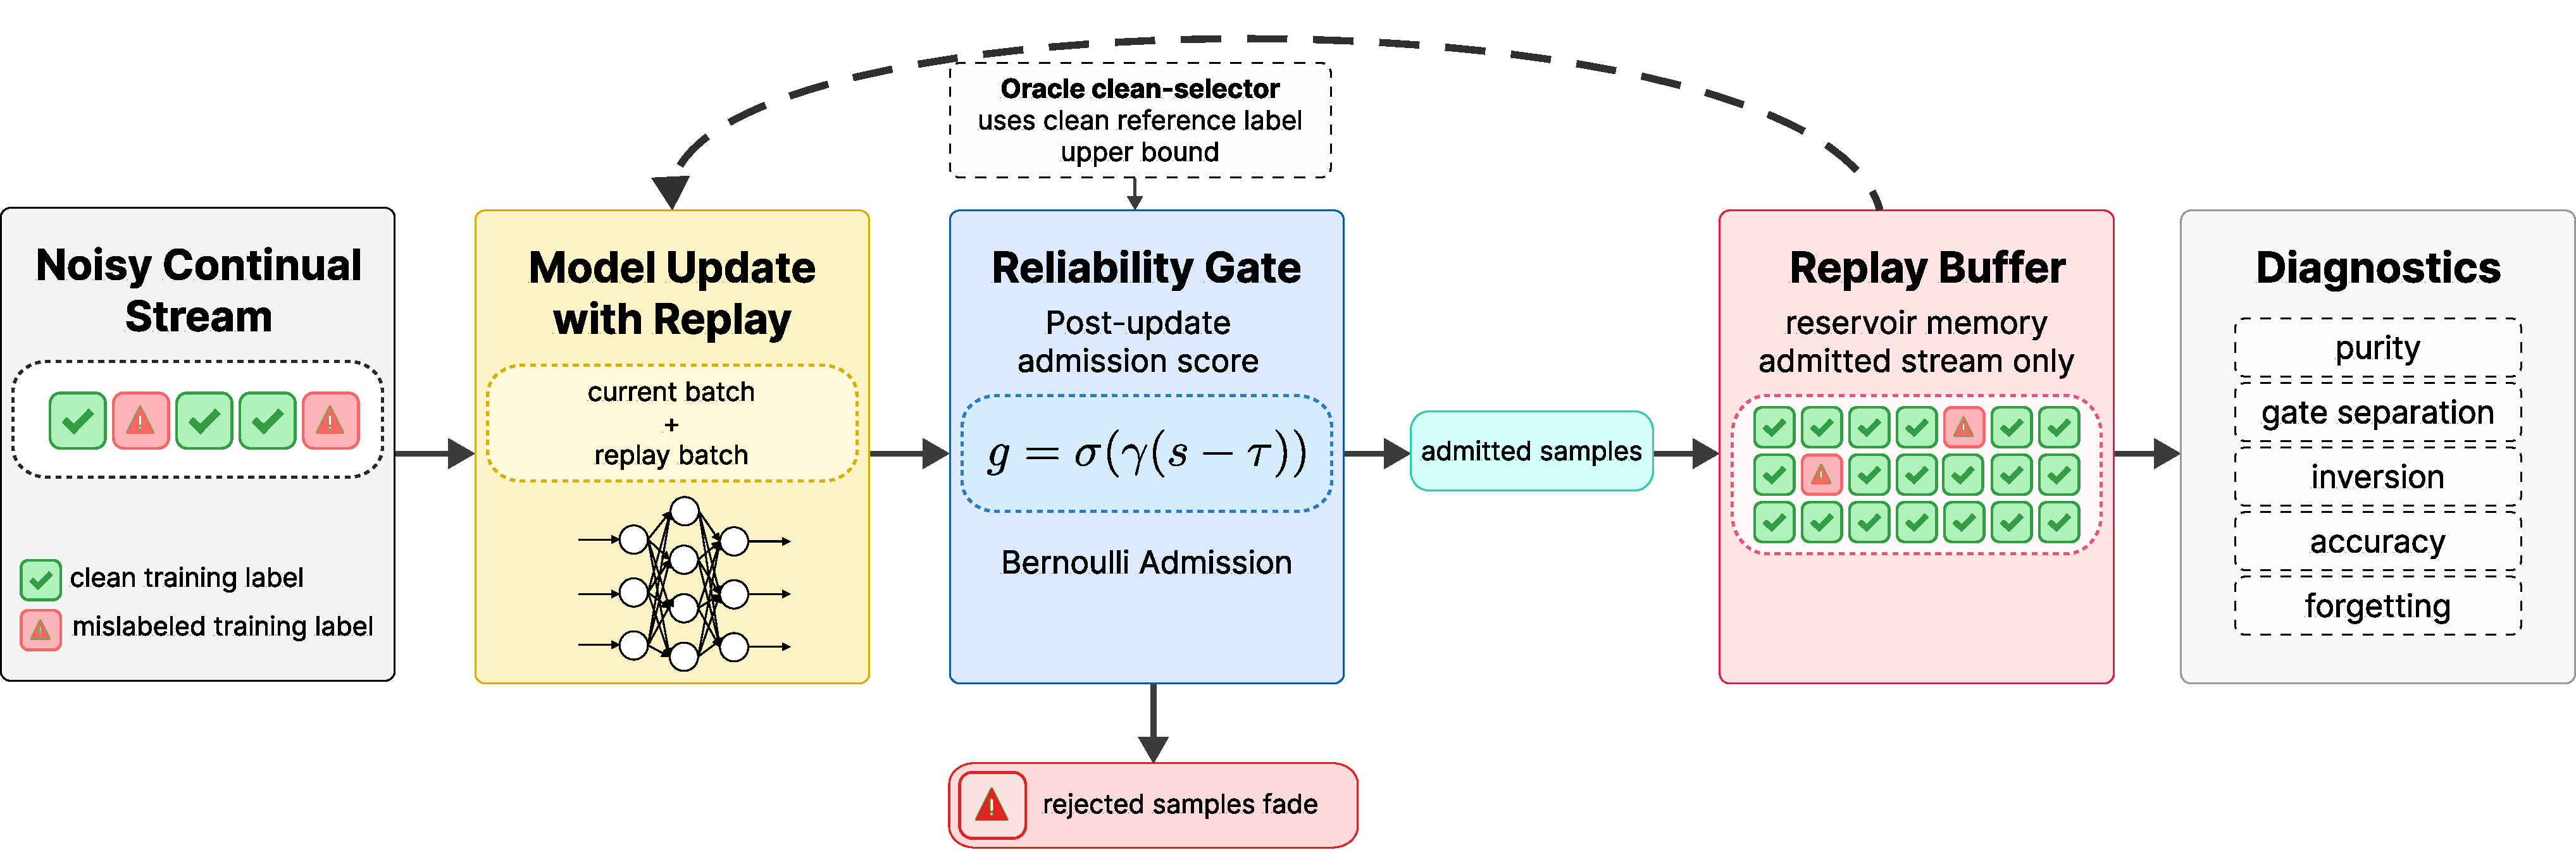
\includegraphics[width=\textwidth]{figs/fig2_reliability_gated_replay.pdf}
\caption{Reliability-gated replay as selective replay admission. A noisy continual stream contains clean and corrupted training labels. At each iteration, the current mini-batch and, when available, a replay mini-batch update the model. The updated model then scores current samples for replay admission through $g=\sigma(\gamma(s-\tau))$. Samples admitted to the replay buffer enter a stabilization substrate because they are rehearsed repeatedly during later updates; rejected samples fade from future training dynamics. The oracle clean-selector admits only clean samples and isolates the effect of buffer purity from endogenous reliability estimation.}
\label{fig:reliability_gated_replay}
\end{figure}

\subsection{Benchmarks, noise, and optimization}

We use two MNIST-family benchmarks as controls: Permuted-MNIST with a single 10-way head and Split-MNIST with few-class heads. The main deep-network benchmarks are Split-CIFAR-10 in the task-incremental setting and Seq-CIFAR-10 in the class-incremental setting, both using ResNet-18 trained from scratch. Split-CIFAR-10 uses five binary tasks with task identity available at test time. Seq-CIFAR-10 uses five sequential two-class tasks with a shared 10-way head and no task identity at test time. Seq-CIFAR-100 uses sequential class-incremental tasks with a shared 100-way head. CIFAR-10N uses the published aggregate and worst human-annotation label sets. CIFAR-10 and CIFAR-10N use five seeds; CIFAR-100 uses three seeds. Test labels are always clean, so reported accuracy is clean-test accuracy. The benchmark taxonomy follows the standard distinction between task-incremental and class-incremental evaluation, and the implementation is compatible with current continual-learning library conventions \cite{VanDeVen2022ThreeTypes,Lomonaco2021Avalanche}.

Training labels are corrupted using symmetric and asymmetric flips at rates up to $80\%$. Symmetric corruption replaces the label with a uniformly sampled incorrect class. Asymmetric corruption uses a fixed class-transition map within the dataset label space and keeps the transition map constant across methods and seeds. For every corrupted example, the clean reference label is retained for analysis only, enabling direct computation of sample correctness, buffer purity, and gate--correctness separation. Models are optimized with Adam, learning rate $10^{-3}$, weight decay 0, batch size 128, and 8 epochs per task. ResNet-18 is trained from scratch without pretrained weights. The replay loss is added to the current-batch loss with unit coefficient. Replay batch size is $m=32$. Standard dataset normalization is applied; no augmentation is used unless specified in the released configuration.


\begin{table}[H]
\centering
\caption{Experimental scope of the replay-admission assay. The grid separates mechanistic controls, deep task-incremental transfer, class-incremental boundary tests, real human-label noise, scale tests, and an external noisy-continual-learning baseline.}
\label{tab:experimental_scope}
\scriptsize
\setlength{\tabcolsep}{3pt}
\renewcommand{\arraystretch}{1.08}
\begin{tabularx}{\linewidth}{@{}p{0.17\linewidth}p{0.17\linewidth}p{0.18\linewidth}p{0.12\linewidth}Y@{}}
\toprule
Benchmark family & Evaluation setting & Noise / label source & Seeds & Role in the assay \\
\midrule
Permuted-MNIST & Continual 10-way control & Synthetic symmetric corruption up to severe noise & Configured runs & Aligned-gate control; tests whether small-loss replay improves learning when clean--noisy separation remains available. \\
Split-MNIST & Few-class task stream & Synthetic symmetric corruption up to severe noise & Configured runs & Inversion control; tests whether severe corruption makes the admission signal anti-aligned with correctness. \\
Split-CIFAR-10 & Task-incremental, ResNet-18, task identity available at test time & Symmetric and asymmetric synthetic corruption & 5 & Deep-network transfer of the power--safety frontier under task-incremental evaluation. \\
Seq-CIFAR-10 & Class-incremental, ResNet-18, shared 10-way head & Symmetric and asymmetric synthetic corruption & 5 & Representation-limited boundary test; separates buffer purification from class-incremental accuracy. \\
CIFAR-10N & Class-incremental, ResNet-18, aggregate and worst human labels & Human annotation noise, approximately $9\%$ and $40\%$ & 5 & Real-noise alignment test; evaluates whether human-label noise remains outside the inversion regime. \\
Seq-CIFAR-100 & Class-incremental, ResNet-18, shared 100-way head & Synthetic symmetric corruption & 3 & Scale test; evaluates whether replay purification transfers to a larger class space. \\
AER baseline & Mammoth \texttt{er\_ace\_aer\_abs}, Seq-CIFAR-10, ResNet-18 & Symmetric $20\%$, symmetric $60\%$, asymmetric $40\%$ & 3 & External noisy-continual-learning baseline for severe-noise replay correction. \\
\bottomrule
\end{tabularx}
\end{table}

For the external noisy-continual-learning baseline, we additionally evaluate AER using the Mammoth-based \texttt{er\_ace\_aer\_abs} protocol on Seq-CIFAR-10 with synthetic corruption. AER is reported on symmetric $20\%$, symmetric $60\%$, and asymmetric $40\%$ label noise over three seeds. The Mammoth implementation reports both Class-IL accuracy and masked Task-IL accuracy from a shared Class-IL head. The masked Task-IL number is reported separately from the native Split-CIFAR-10 task-incremental results, which use separately parameterized task heads.

\begin{table}[H]
\centering
\caption{Frozen gate and baseline hyperparameters.}
\label{tab:hparams}
\small
\begin{tabular}{ll}
\toprule
Method & Hyperparameters \\
\midrule
Small-loss / SPR-style score & $\gamma=3.0$, $\tau_{\mathrm{err}}=1.0$ \\
Confidence & $\gamma=6.0$, $\tau=0.5$ \\
Prediction stability & $\gamma=6.0$, $\tau=0.6$, EMA $\beta=0.6$ \\
Representation stability & $\gamma=6.0$, $\tau=0.5$, $\alpha=2.0$, EMA $\beta=0.6$ \\
Teacher agreement & $\gamma=6.0$, $\tau=0.5$, momentum $0.999$ \\
Co-teach agreement & $\gamma=6.0$, $\tau=0.5$, keep $0.5$, peer lr $10^{-3}$ \\
DER++ & $\alpha=0.5$, $\beta=1.0$ \\
EWC & $\lambda=100$ \\
SI & $\lambda=1$ \\
\bottomrule
\end{tabular}
\end{table}

\subsection{Computational overhead}

Reliability gating adds an admission-scoring step but does not change the replay loss or the base optimizer. For single-model gates such as small-loss, confidence, prediction stability, and representation stability, the additional cost is one no-gradient forward scoring pass over the current mini-batch after the optimizer update. This pass is performed in evaluation mode with BatchNorm statistics frozen only during scoring. The gate does not introduce an additional backward pass.

The memory overhead is limited to the replay buffer and any auxiliary statistics required by the gate. In all experiments, replay buffer capacity is fixed at $M=500$ and replay mini-batch size is at most $m=32$. Prediction-stability and representation-stability gates require exponential moving averages of predictions or representations. Teacher-agreement gates require a momentum teacher, and co-teaching requires a peer model; these variants therefore have higher computational and memory cost than single-model gates.

Clean reference labels are used for diagnostics and for the oracle control. Realizable gates use only the observed training stream. Buffer purity, gate--correctness separation, and oracle admission define the controlled operating regime of the assay; they are not inputs to the deployed gates.

\begin{table}[H]
\centering
\caption{Computational and memory cost of replay-admission variants. The base replay loss and optimizer are unchanged; costs arise from admission scoring and auxiliary state.}
\label{tab}
\scriptsize
\setlength{\tabcolsep}{3pt}
\renewcommand{\arraystretch}{1.08}
\begin{tabularx}{\linewidth}{@{}p{0.20\linewidth}p{0.18\linewidth}p{0.16\linewidth}p{0.22\linewidth}Y@{}}
\toprule
Method & Extra scoring pass & Extra backward pass & Extra state & Cost interpretation \\
\midrule
ER & No & No & Replay buffer only & Reference replay baseline. \\
DER++ & No admission scoring & No additional model & Stored logits / targets & Replay baseline with functional regularization overhead. \\
Small-loss gate & One no-gradient forward pass & No & None beyond buffer & Low overhead; single-model self-scored admission. \\
Confidence gate & One no-gradient forward pass & No & None beyond buffer & Low overhead; label-free self-scored admission. \\
Prediction stability & One no-gradient forward pass & No & Prediction EMA & Low compute, small auxiliary-memory cost. \\
Representation stability & One no-gradient forward pass & No & Representation EMA & Low compute, moderate auxiliary-memory cost if embeddings are stored. \\
Teacher agreement & One no-gradient forward pass & No & Momentum teacher & Moderate memory cost from the teacher model. \\
Co-teaching agreement & Peer forward pass & Peer-model update & Peer model & Highest native-gate cost; agreement can fail when both learners memorize noise. \\
Oracle clean-selector & Not deployable & Not deployable & Clean reference labels & Analysis-only upper bound for clean selective replay. \\
AER & Additional buffer-learning / buffer-forgetting passes & Yes & Mammoth AER state & Strong external baseline; measured overhead is approximately $31\%$ at symmetric $60\%$ noise. \\
\bottomrule
\end{tabularx}
\end{table}

\subsection{Metrics and statistical analysis}

The primary performance metrics are final average accuracy and mean forgetting. Mechanistic metrics are buffer purity, gate--correctness correlation, and gate separation,
\begin{equation}
\Delta = \bar{g}_{\mathrm{correct}}-\bar{g}_{\mathrm{wrong}}.
\end{equation}
A gate is inverted when $\Delta<0$. Time-to-inversion is the first evaluation at which $\Delta$ becomes negative and remains negative for at least two consecutive evaluations. Inversion rate is the fraction of evaluations with $\Delta<0$. Calibration metrics are expected calibration error, Brier score, and negative log likelihood.

Comparisons against ungated ER are paired on condition and seed. We report mean deltas, percentile bootstrap $95\%$ confidence intervals using $10^4$ resamples, paired Wilcoxon signed-rank tests, paired Cohen's $d_z$, and matched-pairs rank-biserial correlations. Benjamini--Hochberg FDR correction is applied within metric families. For the diagnostic claim, we regress accuracy gain over ER on gate separation and buffer purity across gated runs and report Pearson correlation, Spearman correlation, and bootstrap confidence intervals. Paired comparisons are also run against DER++.

\subsection{Predefined operating regimes and power--safety plane}

Before method comparison, we define three operating regimes. The aligned regime is defined by positive gate--correctness separation, $\Delta>0$, meaning that clean samples receive higher replay-admission scores than mislabeled samples. The inverted regime is defined by negative gate--correctness separation, $\Delta<0$, meaning that mislabeled samples receive higher replay-admission scores than clean samples. The representation-limited regime is defined by positive or near-positive separation combined with weak accuracy gain because final performance is dominated by class-incremental interference rather than buffer purity.

The power--safety plane is defined before method comparison. The power axis is the gain over ungated ER in a moderate-noise condition where clean--noisy separation is expected to remain available. The safety axis is the penalty relative to ER in a high-noise condition where self-scored reliability may become anti-aligned after memorization. A gate is favorable when it improves performance in the aligned regime without producing a large penalty in the inverted regime.

\section{Results}

\subsection{Aligned gating}

On Permuted-MNIST, where each task contains many classes and moderate noise preserves a usable clean--noisy loss gap, the small-loss gate improves learning. At $40\%$ symmetric noise, it reaches $0.80$ average accuracy versus $0.72$ for ungated ER while keeping the buffer $94\%$ clean. The pooled accuracy advantage over ER survives FDR correction, with $\Delta=+0.071$ and $d_z=+0.91$. The same gate imposes no measurable cost at $0\%$ noise. This is the regime in which small-loss sample selection works: the endogenous reliability signal remains aligned with sample correctness.

\subsection{Gate inversion}

Under severe or structured corruption, the same gate crosses from adaptive selection into inverted selection. On Split-MNIST with binary heads, as noise rises from $20\%$ to $80\%$, the gate--correctness correlation flips from $+0.91$ to $-0.91$, gate separation flips from $+0.59$ to $-0.59$, and buffer purity collapses from $0.94$ to $0.06$. At $60\%$ noise, accuracy falls below ungated ER, $0.28$ versus $0.33$. The mechanism is direct: once the learner memorizes the corrupted majority, mislabeled examples become low-loss or high-confidence and receive high gate values. The gate then stabilizes error.

The label-free confidence gate defines the opposite corner of the frontier: lower inversion risk with weaker purification. It produces weak clean--noisy separation under high noise but avoids strong inversion. Its separation remains close to zero, while the small-loss gate becomes negative. Under high noise, the confidence gate's separation is $+0.33$ higher than that of the small-loss gate, with paired $p=0.031$. This establishes the core power--safety trade-off: supervised gates are high-gain/high-risk, whereas label-free gates reduce inversion risk at the cost of weaker purification.

\begin{figure}[H]
\centering
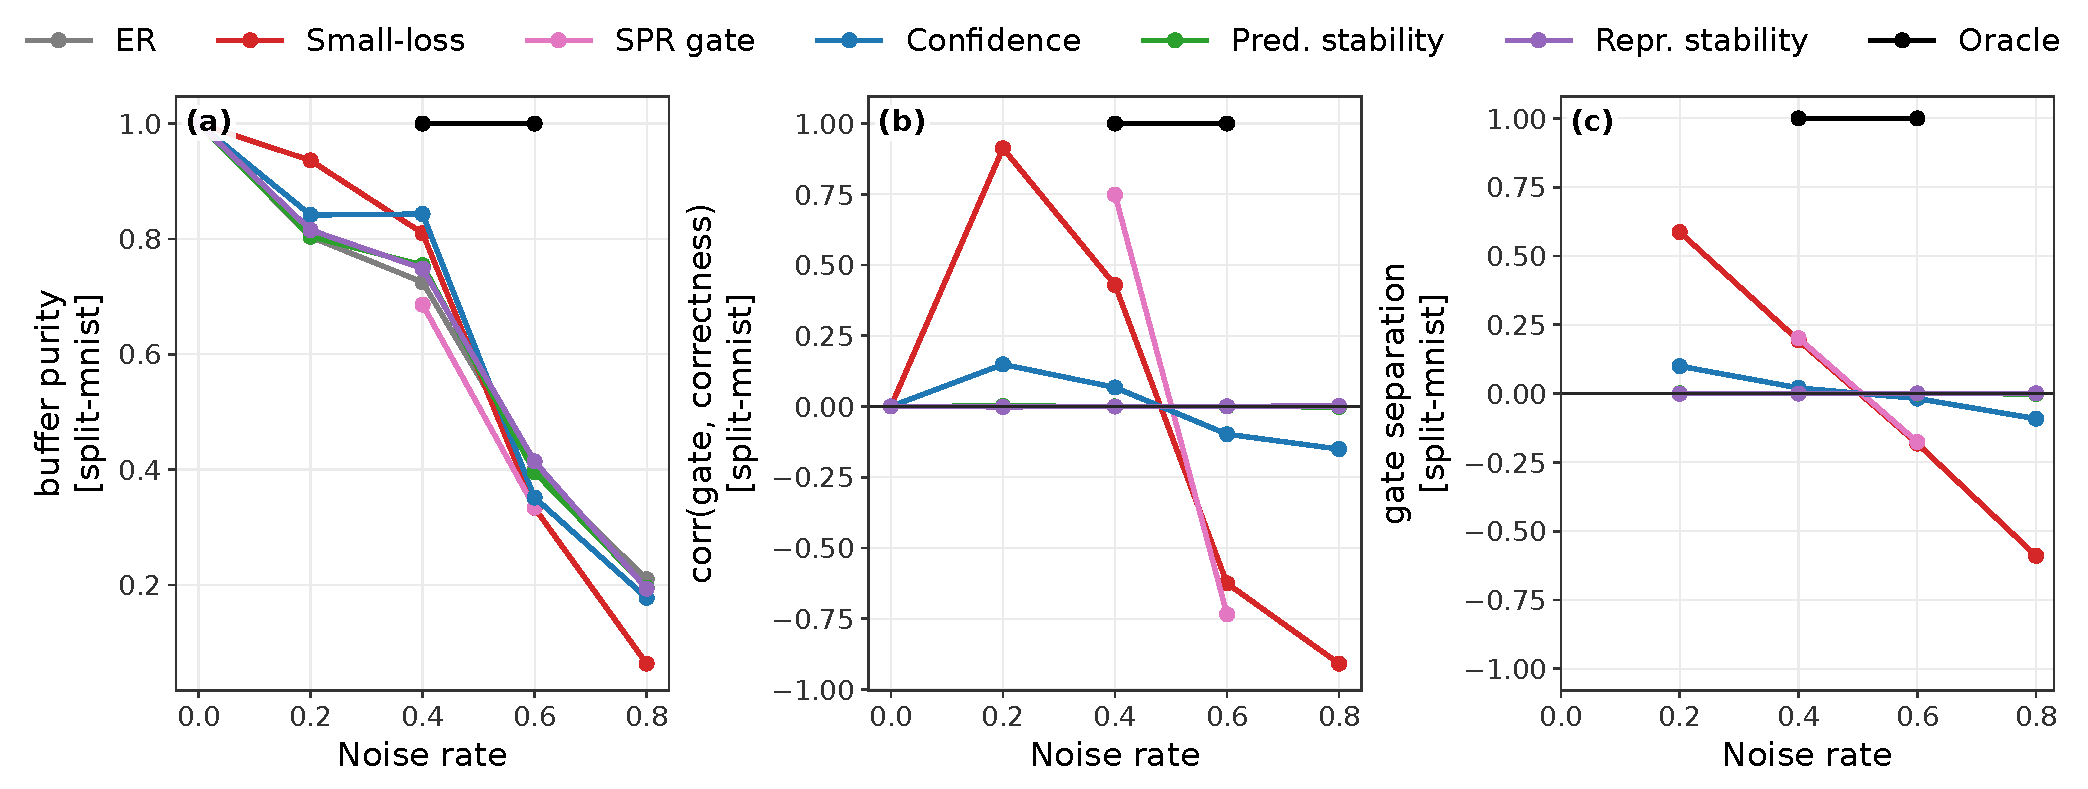
\includegraphics[width=\linewidth]{fig4_buffer_purity_gate_alignment.pdf}
\caption{Buffer purity, gate--correctness correlation, and gate separation as a function of noise rate. Supervised gates lose purity and become negatively aligned under heavy noise, whereas the confidence gate remains close to zero separation.}
\label{fig:purity}
\end{figure}

\begin{figure}[H]
\centering
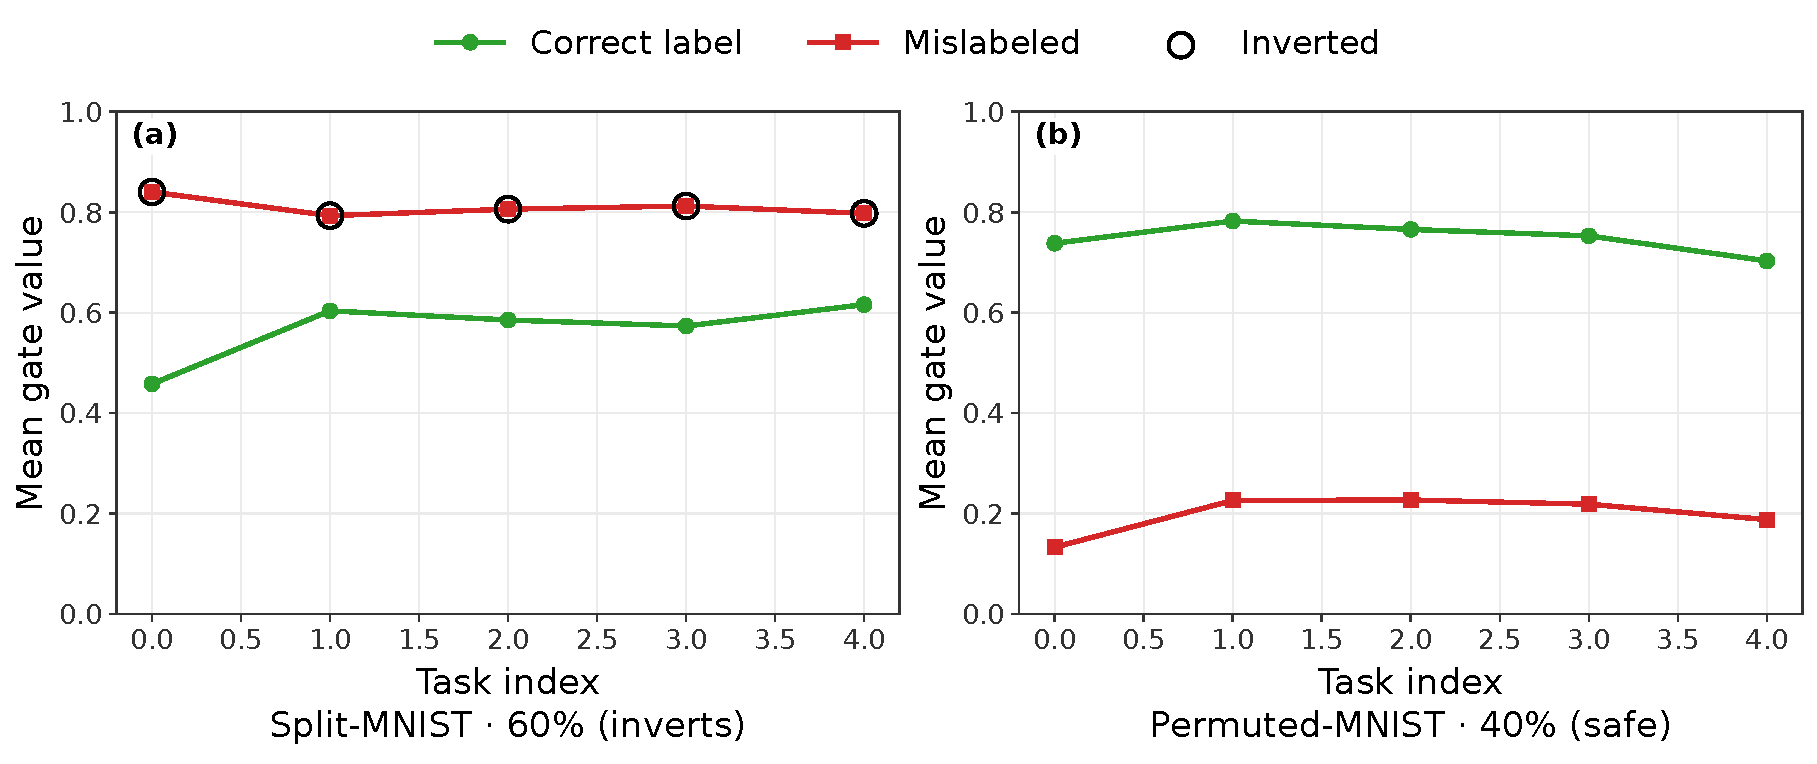
\includegraphics[width=\linewidth]{fig5_memorization_inversion.pdf}
\caption{Gate values assigned to clean and mislabeled samples over tasks. In the high-noise few-class setting, the small-loss gate assigns higher scores to mislabeled samples. In the moderate-noise many-class setting, the same gate preserves healthy separation.}
\label{fig:inversion}
\end{figure}

\subsection{Integrated power--safety frontier}

Using the predefined power--safety plane, each method is summarized by its mean gain over ER across moderate-noise conditions and its worst accuracy penalty relative to ER across high-noise or structured-noise conditions (Fig.~\ref{fig:integrated_power_safety}). This integrated power--safety frontier separates high-power gates that carry large high-noise penalties from safer low-gain gates. Co-teaching gives the largest power but also the largest penalty on the risk axis, consistent with agreement becoming unreliable when models share memorized noise. Small-loss, DER++, EWC, and slow-teacher gates occupy an intermediate region: they provide positive gains, but remain vulnerable when the endogenous reliability signal becomes anti-aligned. Confidence and stability-based gates occupy the safer low-power region. The oracle combines high power with low penalty because it removes the self-scoring bottleneck and admits only clean samples.

This frontier sharpens the mechanism. Replay admission is useful when the gate separates clean from corrupted samples, dangerous when the gate stabilizes mislabeled samples, and bounded when representation-level forgetting dominates the effect of memory purity. The oracle point shows that clean selective replay remains valuable; the distance between the oracle and realizable gates quantifies the cost of estimating reliability from the learner's own state.

\begin{figure}[!htbp] \centering 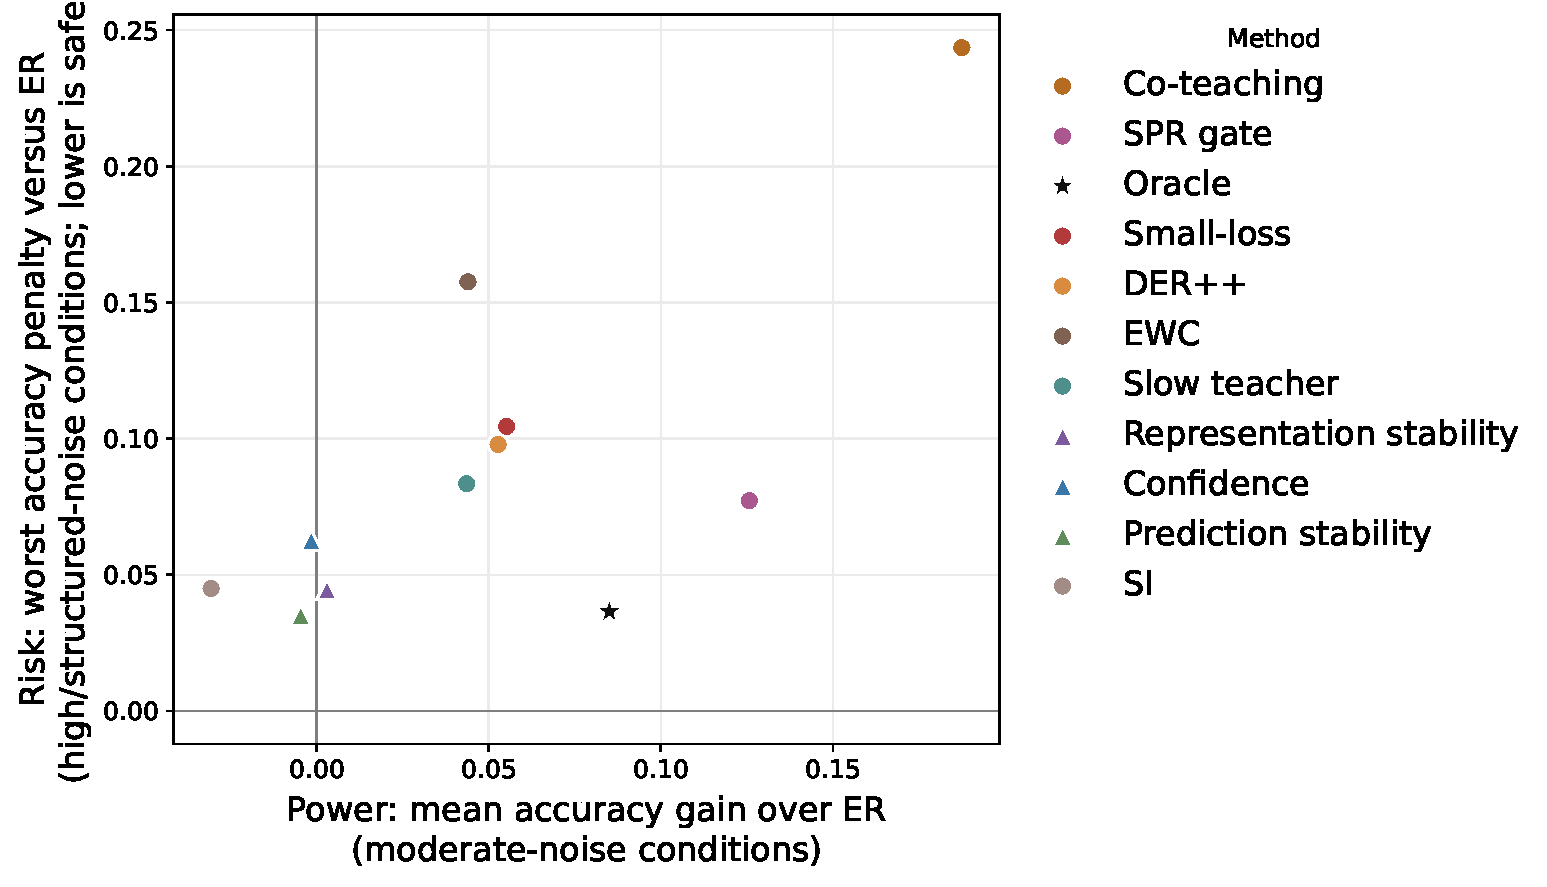
\includegraphics[width=0.96\linewidth]{fig_integrated_power_risk_frontier.pdf} \caption{Integrated power--safety frontier. The $x$-axis shows mean accuracy gain over ER across moderate-noise conditions. The $y$-axis is the risk axis: it shows the worst accuracy penalty relative to ER across high-noise or structured-noise conditions; lower values are safer. High-power supervised gates provide larger gains but carry larger penalties when the reliability signal inverts. Label-free and stability-based gates occupy the safer region. The oracle separates clean replay from endogenous reliability estimation.} \label{fig:integrated_power_safety} \end{figure} \FloatBarrier

\subsection{Predictive gate separation}

Across all gated runs, the accuracy change over ER is strongly related to gate separation. At the run level, with $n=530$ gate-versus-ER pairs, Pearson correlation is $r=+0.74$ and Spearman correlation is $\rho=+0.81$. At the condition-mean level, with one point per benchmark, method, and noise condition, the correlation is $r=+0.80$ over $n=154$ points. A cluster bootstrap resampling whole conditions gives a $95\%$ confidence interval of $[+0.57,+0.84]$. Gate separation also predicts the sign of the effect: the ROC-AUC for classifying whether gating beats ER is $0.85$, and the optimal threshold is $+0.016$, close to the mechanistic crossover at zero separation. A permutation control that shuffles gate-separation values collapses the association to $0.00\pm0.04$, with $p<10^{-3}$.

The predictor is regime-specific. It is strong when buffer purity is the limiting factor, including MNIST ($r=+0.81$) and task-incremental Split-CIFAR-10 ($r=+0.68$). It vanishes in class-incremental CIFAR ($r=-0.26$), where representational forgetting dominates memory contamination. This boundary defines the operating domain of the diagnostic. Gate separation predicts replay payoff when memory purification can affect accuracy. It becomes uninformative when the dominant failure is representational interference.

\subsection{Oracle purity bound} The oracle isolates the effect of replay purity from the limitations of self-scored admission. On CIFAR-10, the oracle lifts buffer purity by $+0.27$ to $+0.39$ over the best realizable gate and improves accuracy by $+0.15$ on Split-CIFAR-10 and $+0.17$ on Seq-CIFAR-10. This establishes that clean selective replay is sufficient to improve learning under the fixed replay mechanism. The oracle removes the self-scoring bottleneck by using the clean reference label. The gap between oracle and realizable gates measures the cost of relying on endogenous signals.

\subsection{CIFAR-10 transfer}

Split-CIFAR-10 with ResNet-18 provides the deep-network task\-in\-cre\-men\-tal instance of the frontier. At moderate noise, the small-loss gate improves performance from $0.673$ for ER to $0.720$ at $20\%$ symmetric noise, a gain of $+4.8$ percentage points observed in all five seeds. This is the adaptive regime of selective replay admission. At high noise, the same gate inverts and falls below ER, reaching $0.430$ versus $0.454$ at $60\%$ symmetric noise. The same replay-admission rule continues to operate, but it now stabilizes the wrong content.

The purification mechanism also transfers to class-incremental Seq-CIFAR-10, but its effect on accuracy is limited by representational interference. These class-incremental experiments test whether buffer purification persists when final accuracy is dominated by representational forgetting rather than memory contamination. At $20\%$ symmetric noise, small-loss buffer purity is $0.96$ versus $0.81$ for ER, with pooled FDR $\Delta=+0.12$ and $d_z=+2.8$. Absolute class-incremental accuracies remain low for all realizable methods. Replay purification succeeds at the buffer level while final accuracy remains governed by absent task identity, classifier competition, and representation drift. The oracle remaining above realizable gates confirms that cleaner memory helps, and also shows that memory purification alone does not solve class-incremental forgetting.

\enlargethispage{3\baselineskip}
\begin{table}[!htbp]
\centering
\caption{Final average accuracy on CIFAR-10 using ResNet-18 over five seeds. Values are mean $\pm$ SD. Split-CIFAR-10 is task-incremental; Seq-CIFAR-10 is class-incremental. The best non-oracle result is shown in bold.}
\label{tab:cifar}
\footnotesize
\setlength{\tabcolsep}{4pt} \renewcommand{\arraystretch}{0.94} \begin{tabular}{llccc}
\toprule
Benchmark & Method & Sym. $20\%$ & Sym. $60\%$ & Asym. $40\%$ \\
\midrule
\multirow{4}{*}{Split-CIFAR-10}
& ER         & $0.673\pm 0.012$ & $\mathbf{0.454\pm 0.017}$ & $0.562\pm 0.022$ \\
& DER++      & $0.687\pm 0.045$ & $0.433\pm 0.017$          & $0.556\pm 0.010$ \\
& Small-loss & $\mathbf{0.720\pm 0.020}$ & $0.430\pm 0.031$ & $\mathbf{0.565\pm 0.023}$ \\
& Oracle     & $0.759\pm 0.011$ & $0.662\pm 0.025$          & $0.710\pm 0.015$ \\
\midrule
\multirow{4}{*}{Seq-CIFAR-10}
& ER         & $0.219\pm 0.014$ & $0.139\pm 0.002$          & $0.125\pm 0.023$ \\
& DER++      & $\mathbf{0.238\pm 0.022}$ & $0.152\pm 0.010$ & $\mathbf{0.137\pm 0.006}$ \\
& Small-loss & $0.214\pm 0.005$ & $\mathbf{0.158\pm 0.015}$ & $0.113\pm 0.016$ \\
& Oracle     & $0.235\pm 0.023$ & $0.196\pm 0.035$          & $0.145\pm 0.033$ \\
\bottomrule
\end{tabular}
\end{table}
\FloatBarrier

\begin{figure}[!htbp]
\centering
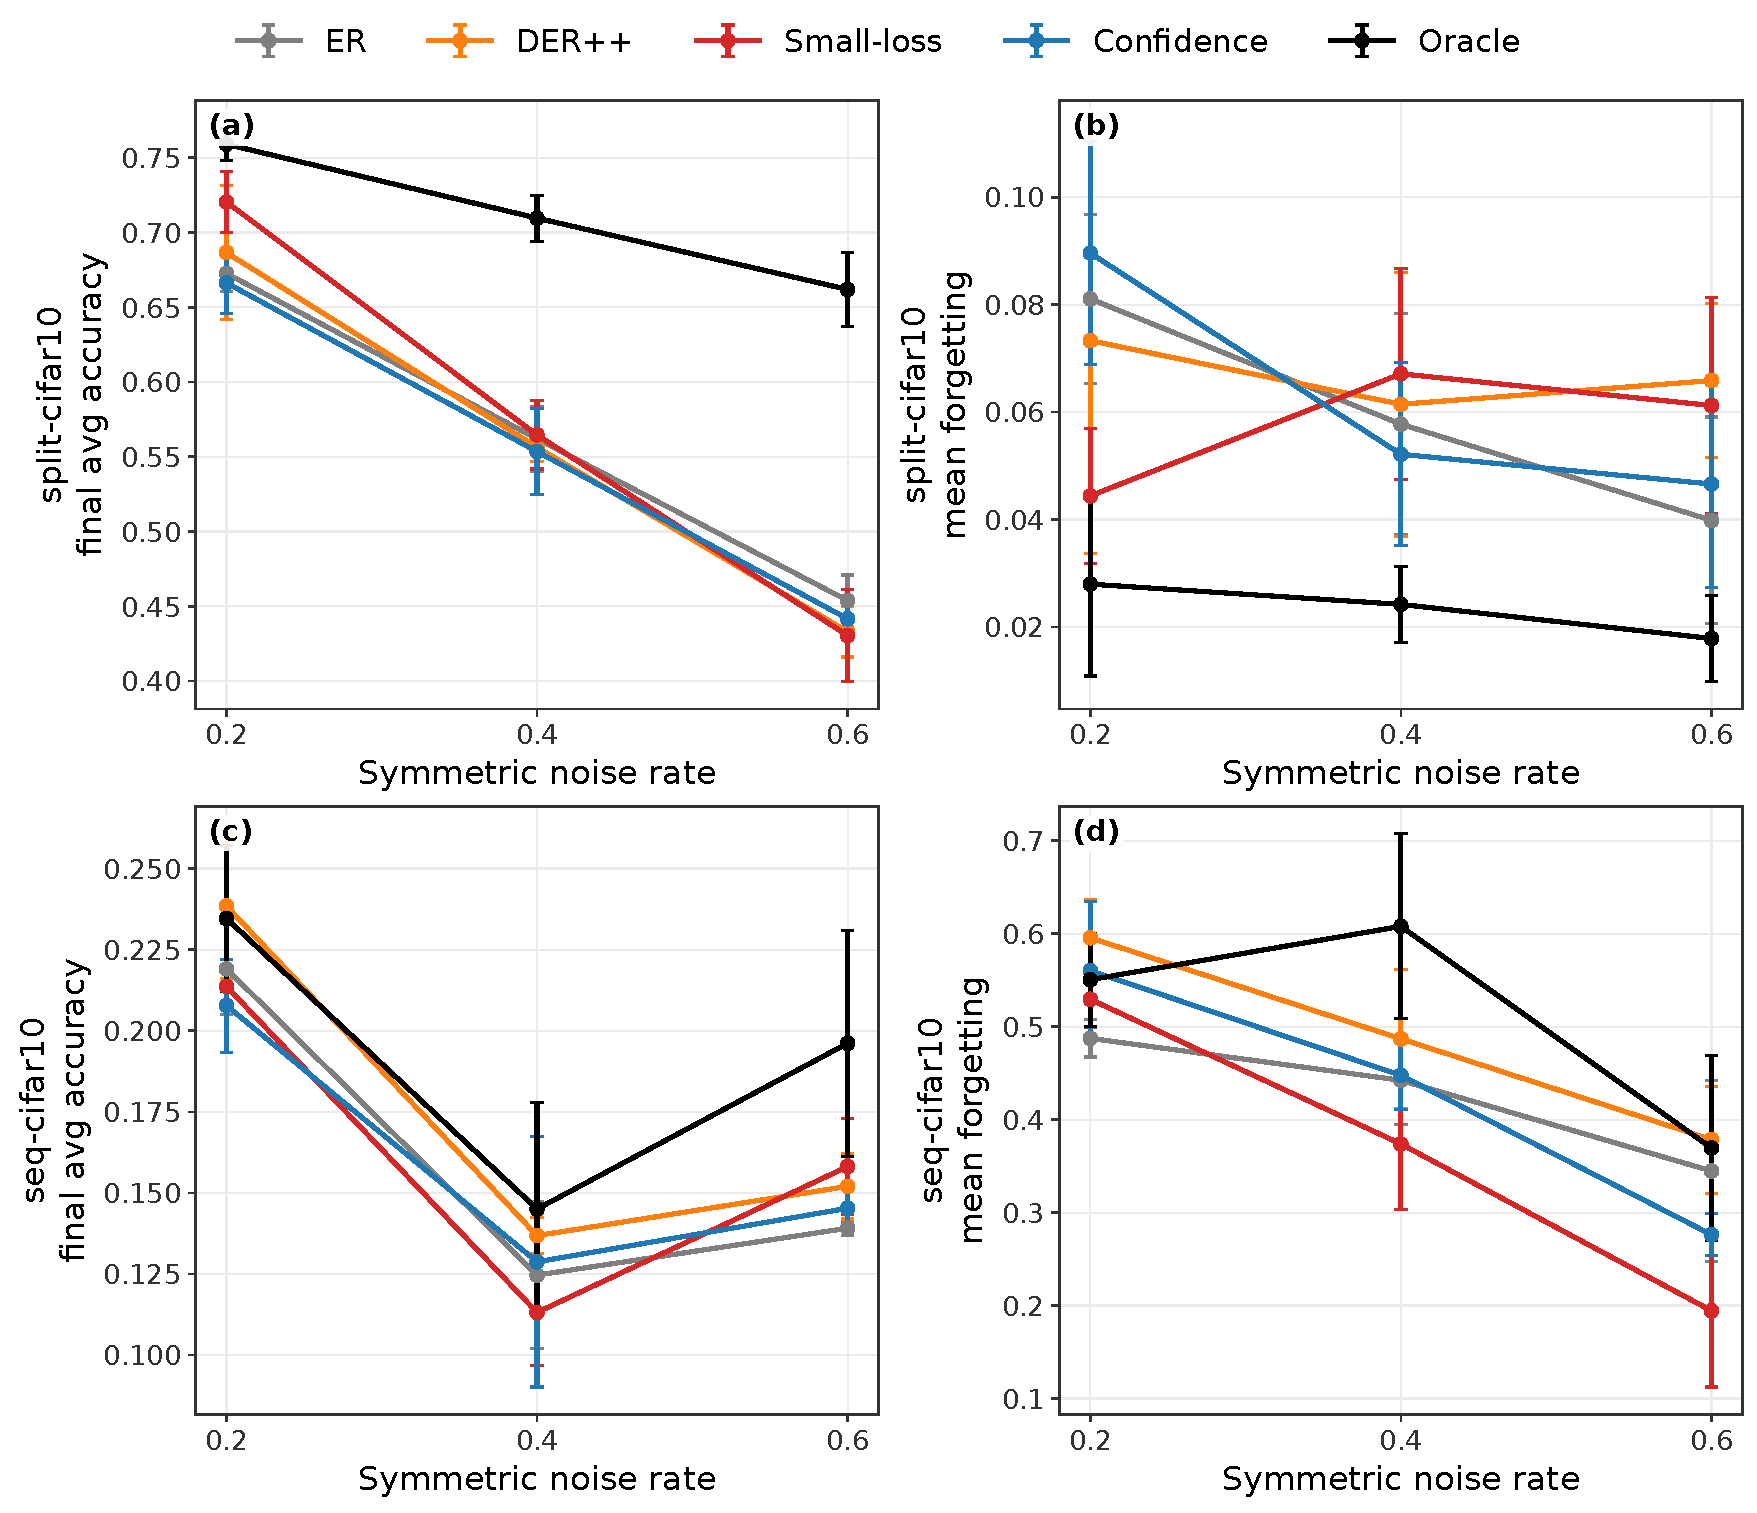
\includegraphics[width=0.98\linewidth]{fig3_main_cifar_benchmark.pdf}
\caption{CIFAR-10 with ResNet-18. Final average accuracy and mean forgetting are shown against symmetric noise for task-incremental and class-incremental settings. The oracle upper-bounds all realizable gates.}
\label{fig:cifar}
\end{figure}
\FloatBarrier

\subsection{Calibration failure}

Calibration exposes a failure mode of self-scored gating. On Split-CIFAR-10 at $20\%$ noise, ECE is lowest for DER++ ($0.061$) and worse for the gates ($0.11$--$0.15$). At the high-confidence end, all methods are over-confident, including the gates that later invert under severe noise. Memorized corrupted samples can become high-confidence and therefore appear reliable to self-scored gates. Calibration therefore diagnoses how memorized corrupted samples become falsely reliable to the gate.

\subsection{CIFAR-10N real-noise regime}

We test the frontier on CIFAR-10N, using the aggregate label set with approximately $9\%$ noise and the worst label set with approximately $40\%$ noise. The supervised gates do not invert under this real annotation noise. Small-loss gate separation remains positive, $+0.51$ for the aggregate set and $+0.12$ for the worst set. Inversion rate is zero. The gate continues to purify the buffer: at the worst set, small-loss buffer purity is $0.81$ versus $0.60$ for ER; at the aggregate set, it is $0.98$ versus $0.91$.

Thus, CIFAR-10N establishes the aligned real-noise regime of the frontier. Its role is to test real-noise alignment and buffer purification, not to optimize Class-IL accuracy. Its label noise exposes replay purification while remaining below the inversion threshold. Because both CIFAR-10N variants are class-incremental, the purity advantage does not translate into a comparable accuracy gain; all methods remain near $0.23$. This matches Seq-CIFAR-10 and reinforces the boundary condition: aligned replay admission is constrained by class-incremental representational forgetting.

\begin{figure}[!htbp]
\centering
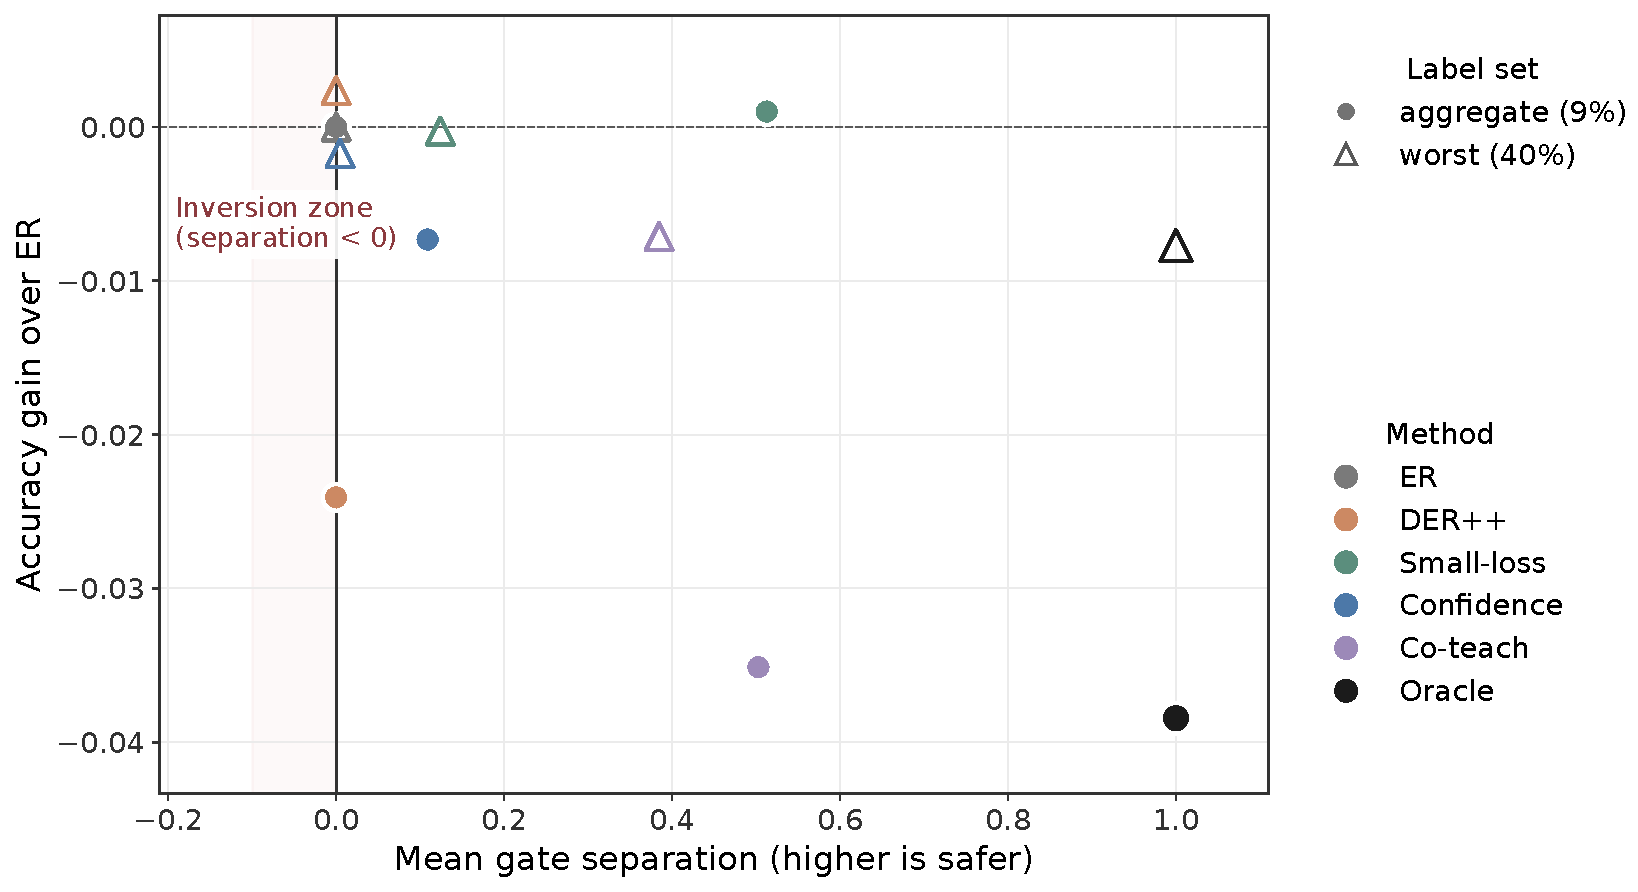
\includegraphics[width=0.96\linewidth]{figA_c10n_frontier.pdf}
\caption{CIFAR-10N power--safety position. Accuracy gain over ER is plotted against mean gate separation. All methods remain outside the inversion zone, indicating benign inversion risk under real human-label noise. This does not imply positive accuracy gain, because these runs are class-incremental and remain representation-limited.}
\label{fig:c10n_frontier}
\end{figure}

\begin{figure}[!htbp]
\centering
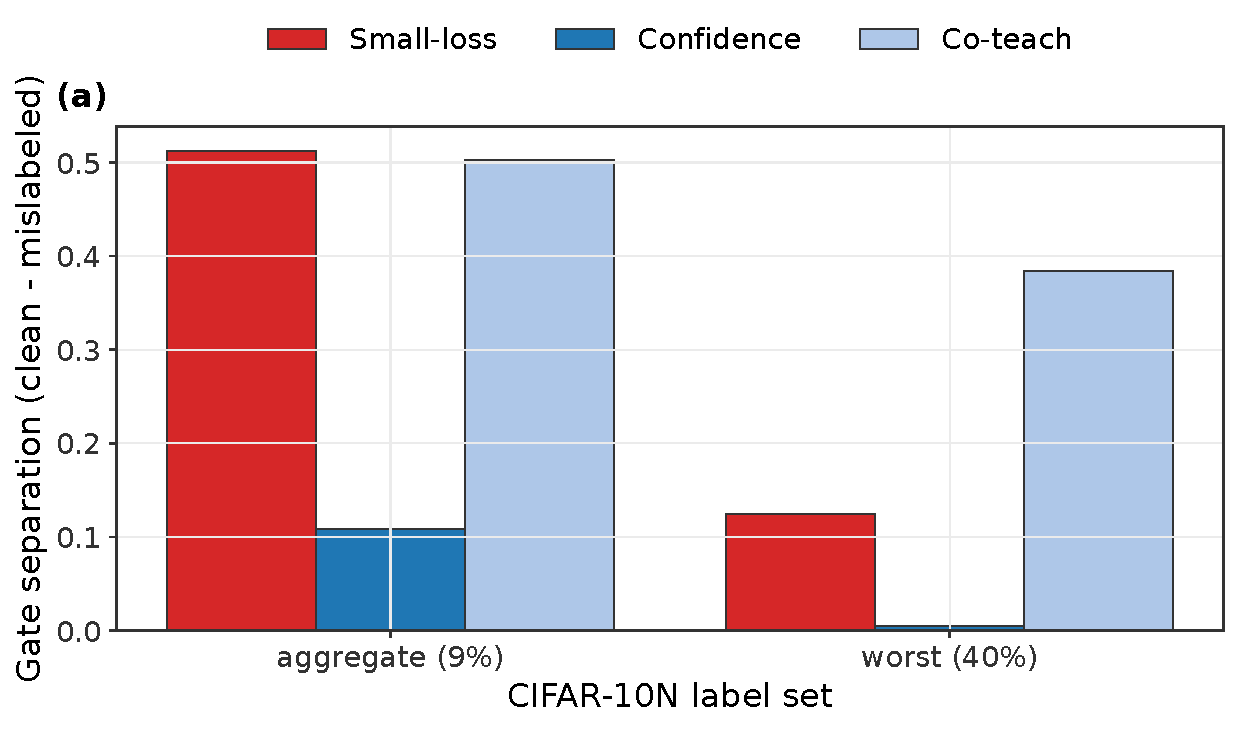
\includegraphics[width=0.92\linewidth]{figB_c10n_separation.pdf}\\[0.4em] 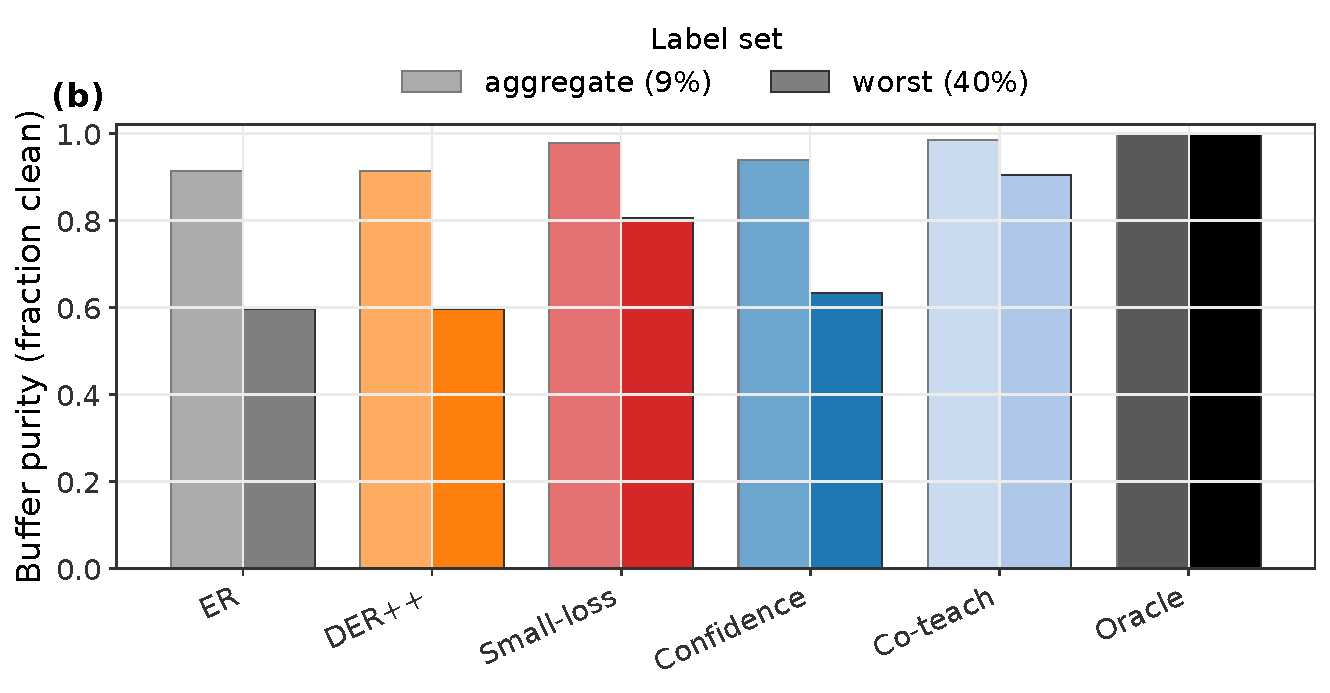
\includegraphics[width=0.96\linewidth]{figC_c10n_purity.pdf}
\caption{CIFAR-10N gate separation and buffer purity. Gate separation remains positive for all gates, and supervised gates purify the buffer above ER and DER++.}
\label{fig:c10n_purity}
\end{figure}
\FloatBarrier

\subsection{CIFAR-100 scale test}

Seq-CIFAR-100 confirms that the purification mechanism transfers to a larger class space. With ResNet-18 over three seeds, the small-loss gate increases buffer purity from $0.82$ to $0.93$ at $20\%$ symmetric noise and from $0.40$ to $0.66$ at $60\%$ symmetric noise. Gate separation remains positive in both regimes. Accuracy gains over ER are small, $+0.010$ and $+0.008$, because class-incremental representational forgetting imposes a strong performance ceiling. As in CIFAR-10, the gate improves replay purity, but the translation from purity to accuracy is constrained by representation capacity and forgetting.

\subsection{Representation-limited replay}
\label{sec:forget}

In class-incremental Seq-CIFAR-10, Seq-CIFAR-100, and CIFAR-10N, final accuracy is governed more by representational forgetting than by buffer contamination. Across class-incremental runs, accuracy correlates more strongly with forgetting ($|r|=0.51$) than with buffer purity ($|r|=0.38$). In a standardized two-predictor regression, the forgetting coefficient dominates the purity coefficient by an approximate factor of four. Memory purification improves the replay substrate but does not resolve inter-class interference, absent task identity, representational overlap, or loss of plasticity in deep continual learning \cite{Dohare2024LossOfPlasticity}.

This defines the computational scope of selective replay admission. Stabilizing cleaner local experience does not resolve representational organization. Gate separation predicts payoff when memory quality is limiting; it becomes uninformative when the limiting variable is class-incremental representation.

\subsection{AER as a strong noisy-continual-learning baseline}

AER provides a strong method-level baseline for the severe-noise failure mode studied here \cite{Millunzi2024AER}. SPR, PuriDivER, and CNLL define closely related noisy continual-learning systems, but they differ in stream assumptions, task-boundary treatment, or semi-supervised machinery. We therefore use AER as the external executable baseline and use the native gates to isolate the admission signal itself. AER actively counteracts the collapse of clean--noisy separation under replay by alternating buffer-learning with buffer-forgetting. We evaluate AER on Seq-CIFAR-10 using the Mammoth-based \texttt{er\_ace\_aer\_abs} implementation under symmetric $20\%$, symmetric $60\%$, and asymmetric $40\%$ label corruption.

\begin{table}[htbp]
\centering
\caption{AER external baseline on Seq-CIFAR-10 with ResNet-18. Results are mean $\pm$ dispersion across seeds. Class-IL is the unmasked class-incremental result. Masked Task-IL is reported by the Mammoth protocol from a shared Class-IL head.}
\label{tab:aer_external}
\small
\begin{tabularx}{\textwidth}{l >{\centering\arraybackslash}X >{\centering\arraybackslash}X c}
\toprule
Condition & Class-IL accuracy & Masked Task-IL accuracy & Runtime \\
\midrule
AER, symmetric $20\%$ & $50.20 \pm 0.90$ & $85.68 \pm 0.34$ & $2707$ s \\
AER, symmetric $60\%$ & $35.63 \pm 1.59$ & $77.84 \pm 1.10$ & $2779$ s \\
AER, asymmetric $40\%$ & $43.86 \pm 1.55$ & $83.83 \pm 1.38$ & $2124$ s \\
Bridge ER, symmetric $60\%$ & $17.47 \pm 0.18$ & $63.55 \pm 1.08$ & $2128$ s \\
\bottomrule
\end{tabularx}
\end{table}

In the severe-corruption regime, AER provides the strongest evidence that preserving clean--noisy separation improves replay performance. At symmetric $60\%$ noise, it increases Class-IL accuracy from $17.47\%$ to $35.63\%$, a gain of $18.16$ percentage points. It also increases masked Task-IL accuracy from $63.55\%$ to $77.84\%$, a gain of $14.29$ percentage points. The measured runtime overhead at symmetric $60\%$ is approximately $31\%$.

AER improves performance by preserving clean replay under severe corruption. This result reinforces the central finding: replay quality depends on alignment between the admission signal and sample correctness. Positive separation marks useful replay admission. Negative separation marks corrupted replay admission. Representational forgetting marks the regime where memory purity no longer determines final accuracy.

\subsection{Robustness controls}

The central relation remains stable across complementary analyses. At the condition-mean level, the correlation between gate separation and accuracy gain is $r=+0.80$. A cluster bootstrap resampling whole conditions gives a $95\%$ confidence interval of $[+0.57,+0.84]$. Leave-one-benchmark-out analyses preserve the relation when CIFAR-10, CIFAR-10N, or CIFAR-100 is removed and weaken it only when MNIST is removed, consistent with the regime dependence above. A permutation control that shuffles gate-separation values collapses the association to chance level with $p<10^{-3}$. Gate--correctness separation is therefore a reliable predictor of replay payoff in regimes where memory purity constrains performance.

Matched-admission random gates preserve the empirical admission rate of the real gates while removing reliability-based selection. These controls isolate sample selection from admission quantity. Clean-only admission-matched oracle gates separate replay purity from admission count. Threshold grids test gate sharpness and cutoff dependence. Buffer-size grids test memory-capacity dependence.

The same regime structure persists across these controls. When gate--correctness separation is positive, selective admission improves replay purity and can improve accuracy. When separation becomes negative, selective admission stabilizes corrupted supervision. When class-incremental interference dominates, buffer purification remains visible but final accuracy is controlled by representational forgetting. Integrated power--safety summaries across noise levels reproduce the same frontier: high-power supervised gates deliver the largest gains when aligned and the largest penalties on the risk axis when their reliability signal inverts; safer gates reduce inversion risk while providing weaker purification.

\subsection{Mechanistic control summary}
The control set maps each empirical pattern to a specific component of the replay-admission mechanism. Table~\ref{tab:control_summary} gives the compact evidence map.

\begin{table}[t]
\centering
\caption{Compact evidence map for the replay-admission mechanism.}
\label{tab:control_summary}
\small
\renewcommand{\arraystretch}{1.2}
\begin{tabularx}{\linewidth}{%
  >{\raggedright\arraybackslash}p{0.22\linewidth}%
  >{\raggedright\arraybackslash}p{0.43\linewidth}%
  >{\raggedright\arraybackslash}X}
\toprule
\textbf{Control} & \textbf{Outcome} & \textbf{Conclusion} \\
\midrule
Ungated ER and matched-random gates &
Purity tracks stream corruption, and rate-matched random admission removes reliability-based selection. &
Replay quantity alone does not explain the gains. \\
\midrule
Small-loss and confidence gates &
Small-loss gives high gain when aligned but inverts under severe noise; confidence remains lower-gain and lower-risk. &
The power--safety frontier follows from gate--correctness alignment. \\
\midrule
Oracle and oracle-thinned gates &
Clean-only replay improves purity and accuracy beyond realizable gates. &
Clean selective replay is sufficient to improve learning under the fixed mechanism, and the oracle gap measures self-scoring cost. \\
\midrule
AER and class-incremental CIFAR &
AER improves severe-noise Seq-CIFAR-10, while CIFAR-10N and CIFAR-100 show purity gains with limited accuracy gains. &
Preserving clean--noisy separation helps, but representational forgetting bounds the payoff. \\
\bottomrule
\end{tabularx}
\end{table}

Together, these controls support a single mechanism: selective replay admission helps when gate--correctness separation is positive, harms when it becomes negative, and loses predictive value when representational forgetting dominates buffer contamination.

\section{Discussion}

Reliability-gated replay exposes replay admission as a control point for memory quality. Stored examples do not merely occupy a buffer; they receive repeated gradient influence during later updates. Admission therefore determines which examples become durable components of training. When the gate remains aligned with useful experience, selective admission improves the replay substrate. When the gate becomes anti-aligned, the same mechanism stabilizes damaging samples. When performance is controlled by representational interference, selective replay admission alone does not determine accuracy.

Replay admission has three operating modes. It improves learning by preferentially retaining clean samples. It harms learning by repeatedly rehearsing mislabeled samples. It becomes weakly predictive when class-incremental interference dominates memory contamination. Gate--correctness separation and buffer purity expose these modes directly.

The power--safety frontier follows from this mechanism. Supervised gates achieve high gain because they exploit the training target directly. The same dependence makes them vulnerable once the learner memorizes corrupted targets. Label-free gates reduce strong inversion but provide weaker purification. The oracle clean-selector isolates the performance effect of buffer purity under the fixed replay mechanism and quantifies the cost of endogenous reliability estimation. Method-level systems such as SPR, PuriDivER, and AER preserve or restore the clean--noisy separation that simple self-scored gates lose under difficult regimes \cite{Kim2021SPR,Bang2022PuriDivER,Millunzi2024AER}.

The class-incremental experiments define the second operating regime. In Seq-CIFAR-10, CIFAR-10N, and Seq-CIFAR-100, positive gate separation and higher buffer purity do not translate into proportional accuracy gains because representational forgetting dominates memory contamination. This result matches broader analyses of class-incremental learning, where absent task identity, inter-class competition, representation drift, and plasticity loss dominate memory quality alone \cite{Masana2023ClassIncrementalSurvey,VanDeVen2022ThreeTypes,Dohare2024LossOfPlasticity}. Selective replay admission controls the replay substrate; class-incremental learning also requires representational organization.

\subsection{Operating regimes}

The power--safety frontier organizes reliability-gated replay into three operating regimes. In the aligned regime, the replay-admission signal assigns higher gate values to clean samples than to corrupted samples. Buffer purity increases, replay payoff is positive, and selective replay admission is adaptive. This regime appears in Permuted-MNIST at moderate noise, task-incremental Split-CIFAR-10 at moderate noise, and CIFAR-10N real human-label noise.

In the inverted regime, the learner assigns higher gate values to corrupted samples than to clean samples. Buffer purity collapses, replay repeatedly reinforces mislabeled targets, and selective replay admission becomes maladaptive. This regime appears under severe or structured synthetic corruption, where memorized mislabeled samples become low-loss or high-confidence.

In the representation-limited regime, the gate remains aligned and buffer purity improves, but accuracy is governed by class-incremental interference. Seq-CIFAR-10, CIFAR-10N, and Seq-CIFAR-100 show this regime. Cleaner buffers confirm successful selective replay admission, while final accuracy is controlled by inter-class competition, absent task identity, classifier bias, and representation drift.

Gate--correctness separation, buffer purity, and oracle admission expose these regimes. Realizable gates use only the observed training labels and endogenous model signals. The oracle clean-selector isolates the effect of replay purity under the fixed replay mechanism, and the oracle gap measures the cost of self-scored replay admission. The operating regimes therefore identify when reliability-gated replay is useful, when it is dangerous, and when it is not the limiting factor.

\subsection{Scope of the diagnostic}

Gate--correctness separation is a diagnostic for replay admission, not a complete solution to continual learning. Its domain is the regime in which memory quality constrains later performance. In that regime, positive separation identifies adaptive replay admission, negative separation identifies maladaptive replay admission, and the oracle gap measures the cost of endogenous self-scoring. When final accuracy is instead dominated by class-incremental representation, cleaner memory remains mechanistically meaningful but no longer determines the final accuracy. This is the operating boundary exposed by Seq-CIFAR-10, CIFAR-10N, and Seq-CIFAR-100. Strong noisy-continual-learning methods such as AER can improve severe-noise performance by actively preserving or restoring clean--noisy separation, whereas reliability-gated replay isolates the admission signal that those corrective mechanisms must maintain.

The resulting design principle is conditional replay control. Binary buffer admission is the simplest implementation. More general mechanisms can adjust replay residence time, replay weight, feature plasticity, logit anchoring, or local learning rates according to the measured alignment of the admission signal. Examples with reliable alignment receive stronger or longer replay influence. Uncertain examples receive weaker or delayed replay influence. Anti-aligned regimes trigger corrective dynamics such as forgetting, re-separation, relabeling, or alternate replay.

\section{Conclusion}

Reliability-gated replay controls which examples continue to shape future learning through repeated rehearsal. The learner does not merely store past samples; it determines which samples enter the replay substrate and acquire repeated gradient influence. The central claim is computational: replay admission is beneficial when the reliability signal is aligned with useful experience, harmful when it is anti-aligned, and insufficient when representational forgetting dominates memory purity.

The results establish a power--safety frontier. When the gate remains aligned with reliable experience, selective admission purifies memory and improves learning. When severe or structured corruption makes the reliability signal anti-aligned, the same mechanism stabilizes damaging experience and becomes maladaptive. When representational forgetting dominates, cleaner replay remains mechanistically successful but no longer controls accuracy.

Gate--correctness separation identifies these regimes. Positive separation marks adaptive replay admission, negative separation marks maladaptive replay admission, and near-zero separation marks an inert gate. The oracle clean-selector isolates the effect of buffer purity and shows that clean selective replay is sufficient under the fixed replay mechanism, while the oracle gap measures the cost of endogenous self-scoring. Existing noisy-replay methods such as SPR, PuriDivER, CNLL, and AER engineer replay under contamination. The present contribution identifies the admission signal that these systems preserve or restore. Continual-learning systems should regulate replay conditionally: strengthen it when endogenous reliability is aligned, weaken it when reliability is uncertain, and correct it when the signal becomes anti-aligned.

\appendix

\section{Supplementary trajectory and external-baseline analyses}

\subsection{Task-wise CIFAR trajectories}

Figure~\ref{fig:supp_taskwise_cifar} shows task-wise accuracy trajectories for Split-CIFAR-10 and Seq-CIFAR-10 under symmetric $20\%$ and $60\%$ label noise. The task-incremental Split-CIFAR-10 trajectories preserve substantially higher accuracy across tasks, whereas the class-incremental Seq-CIFAR-10 trajectories collapse rapidly after the first task. This temporal pattern supports the representation-limited interpretation: replay purification can improve the stored sample distribution, but class-incremental interference can still dominate final accuracy.

\begin{figure}[H]
\centering
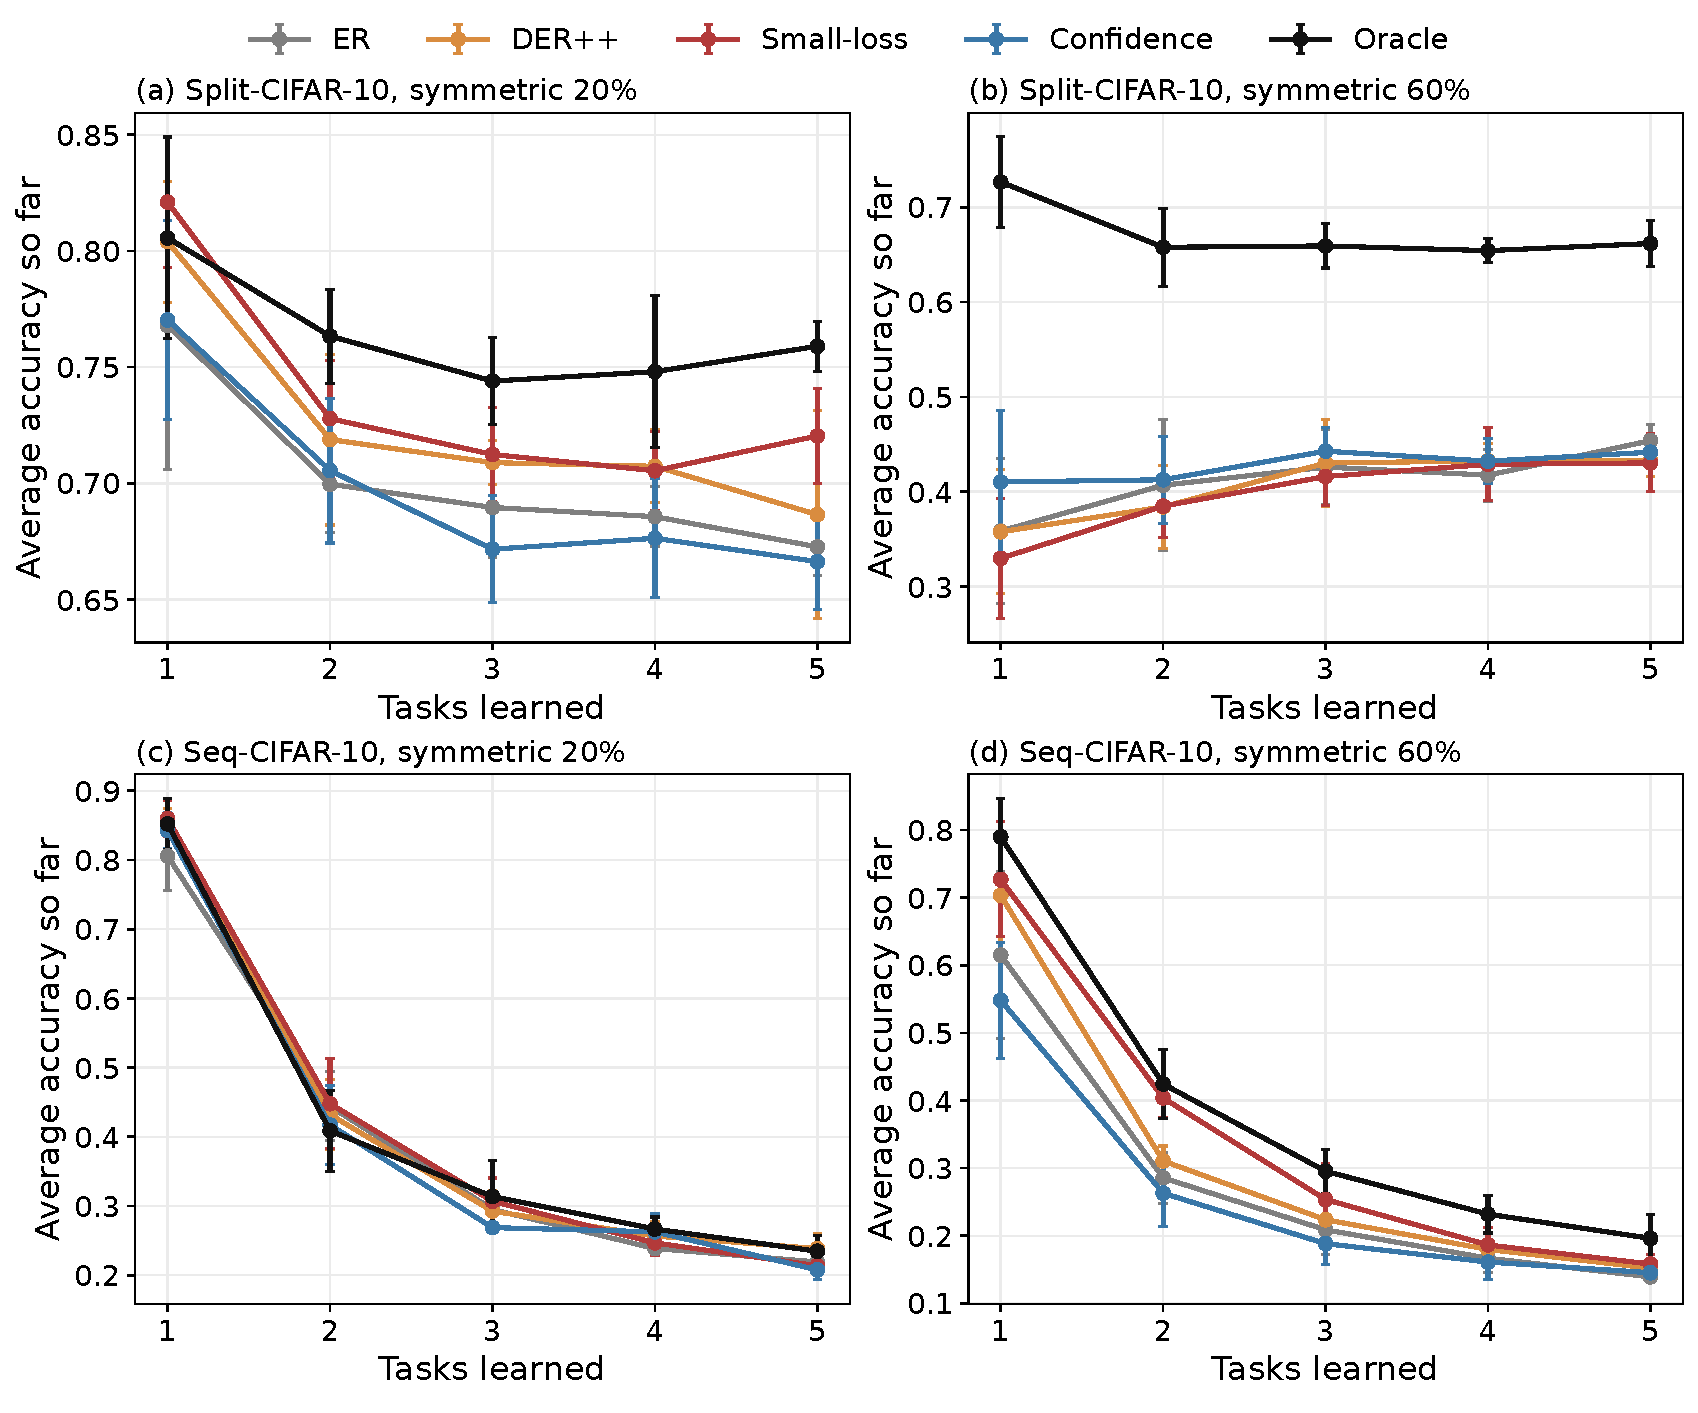
\includegraphics[width=\linewidth]{figS1_taskwise_cifar_trajectories.pdf}
\caption{Task-wise accuracy trajectories on Split-CIFAR-10 and Seq-CIFAR-10. Split-CIFAR-10 preserves higher accuracy across tasks, whereas Seq-CIFAR-10 shows rapid degradation after early tasks, consistent with class-incremental representational interference. Error bars denote variability across seeds.}
\label{fig:supp_taskwise_cifar}
\end{figure}

\subsection{External AER baseline}

Figure~\ref{fig:supp_aer_baseline} summarizes the external AER baseline on Seq-CIFAR-10. AER reaches $50.20\pm1.10\%$ Class-IL accuracy and $85.68\pm0.42\%$ masked Task-IL accuracy at symmetric $20\%$ noise, $35.63\pm1.95\%$ Class-IL accuracy and $77.84\pm1.35\%$ masked Task-IL accuracy at symmetric $60\%$ noise, and $43.86\pm1.90\%$ Class-IL accuracy and $83.83\pm1.69\%$ masked Task-IL accuracy at asymmetric $40\%$ noise. At symmetric $60\%$ noise, the ER bridge baseline reaches $17.47\pm0.25\%$ Class-IL accuracy and $63.55\pm1.52\%$ masked Task-IL accuracy. AER therefore improves the severe-noise Class-IL result by $18.16$ percentage points and the masked Task-IL result by $14.30$ percentage points. Runtime increases from $2128$ s for the ER bridge to $2779\pm90$ s for AER, corresponding to an approximately $31\%$ overhead.

\begin{figure}[H]
\centering
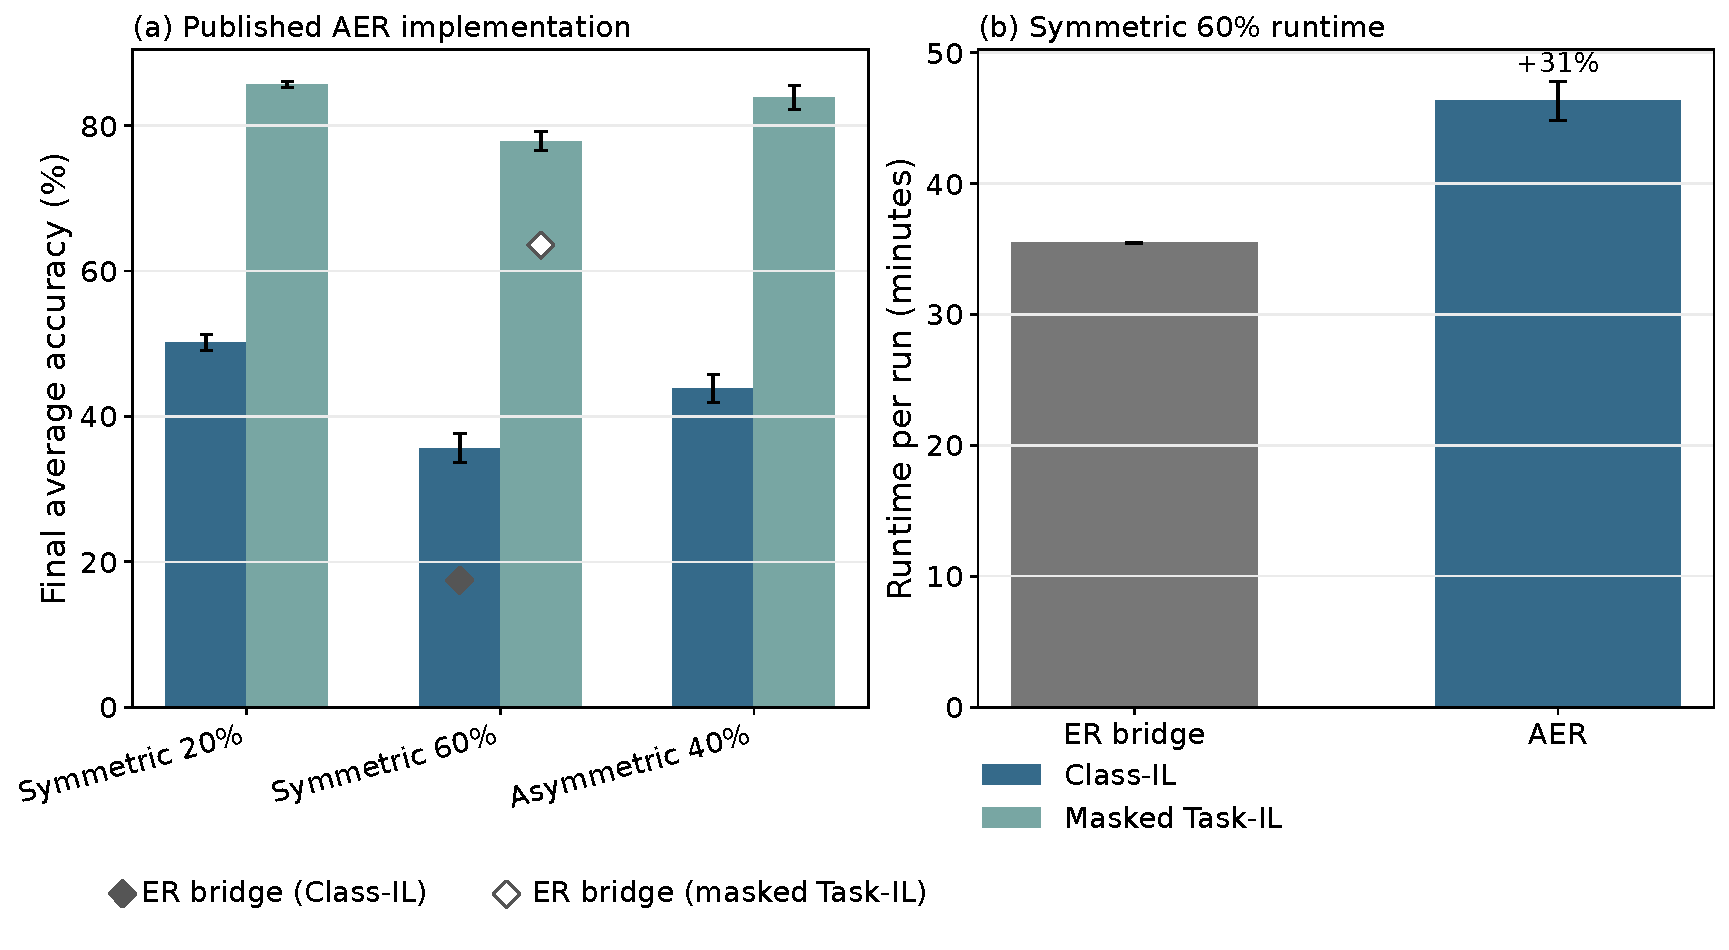
\includegraphics[width=\linewidth]{figS2_aer_external_baseline.pdf}
\caption{External AER baseline on Seq-CIFAR-10. AER improves both Class-IL and masked Task-IL accuracy under synthetic label corruption. At symmetric $60\%$ noise, AER improves Class-IL accuracy by $18.16$ percentage points and masked Task-IL accuracy by $14.30$ percentage points relative to the ER bridge baseline, with an approximately $31\%$ runtime overhead. Error bars denote variability across seeds.}
\label{fig:supp_aer_baseline}
\end{figure}

\section*{CRediT authorship contribution statement}

\textbf{Marlon Malheiros:} Conceptualization, Methodology, Software, Validation, Formal analysis, Investigation, Data curation, Visualization, Writing -- original draft, Writing -- review and editing.

\textbf{Antonio Pereira:} Conceptualization, Methodology, Supervision, Project administration, Resources, Writing -- original draft, Writing -- review and editing.

\section*{Declaration of competing interest}

The authors declare that they have no known competing financial interests or personal relationships that could have appeared to influence the work reported in this paper.

\section*{Funding}

This research received no specific grant from any funding agency in the public, commercial, or not-for-profit sectors.

\section*{Data and code availability}

Code, configuration files, aggregated results, and figure-generation scripts will be made available in a public repository at \url{INSERT_REPOSITORY_URL}. Public benchmark datasets were obtained from their original sources; clean reference labels were used only for diagnostics and oracle controls, not by realizable gates.

\section*{Acknowledgements}

None.

\section*{Supplementary material}

Supplementary material associated with this article includes additional benchmark results, robustness controls, calibration analyses, and implementation details for the replay-admission assay.

\begingroup
\sloppy
\bibliographystyle{elsarticle-num-names}
\bibliography{references}
\endgroup

\end{document}
